% Paquets généraux
\documentclass[a4paper,12pt,titlepage,twoside]{article}
\usepackage[T1]{fontenc}
\usepackage[utf8]{inputenc}
\usepackage[french]{babel}
\addto\captionsfrench{%
  \renewcommand{\tablename}{Tableau}%
}
\usepackage[gen]{eurosym}
%\usepackage[dvips]{graphicx}
\usepackage{fancyhdr}
\usepackage{pdfpages} 
\usepackage{multido}
\usepackage{hyperref}
%\usepackage{textcomp}
\usepackage{schemabloc}
\usepackage[bitstream-charter]{mathdesign}
\usepackage{array}
\newcolumntype{P}[1]{>{\centering\arraybackslash}p{#1}}

\newcommand{\id}{54}
\newcommand{\nom}{Liaisons mécaniques}
\newcommand{\sequence}{04}
\newcommand{\num}{01}
\newcommand{\type}{TP}
\newcommand{\descrip}{Modélisation d'un solide. Comportement des liaisons mécaniques. Modéliser les mécanismes du laboratoire par un schéma cinématique, paramétré.}
\newcommand{\competences}{A3-C4: Analyse d'architecture et de comportement \\ &  Mod1-C1: Isolement d'un solide ou d'un système de solides \\ &  Mod2-C10-1: Modèle de solide indéformable \\ &  Mod2-C11: Modélisation géométrique et cinématique des mouvements entre solides indéformables \\ &  Mod2-C12: Modélisation cinématique des liaisons entre solides \\ &  Mod2-C15: Modélisation des actions mécaniques \\ &  Rés-C6: Utilisation d'un solveur ou d'un logiciel multi physique \\ &  Com1-C1: Différents descripteurs introduits dans le programme \\ &  Com2-C4: Outils de communication}
\newcommand{\nbcomp}{9}
\newcommand{\systemes}{Plateforme Stewart}
\newcommand{\systemessansaccent}{Plateforme Stewart}
\newcommand{\ilot}{2}
\newcommand{\ilotstr}{02}
\newcommand{\dossierilot}{\detokenize{Ilot_02 Plateforme Stewart}}
\newcommand{\imageun}{Plateforme}

\newcommand{\urlsysteme}{\href{https://www.costadoat.fr/systeme/57}{Ressources système}}
\newcommand{\matlabsimscape}{\href{https://github.com/Costadoat/Sciences-Ingenieur/raw/master/Systemes/Plateforme Stewart/Plateforme_Stewart_Simscape.zip}{Modèle Simscape}}
\newcommand{\solidworks}{\href{https://github.com/Costadoat/Sciences-Ingenieur/raw/master/Systemes/Plateforme Stewart/Plateforme_Stewart_Solidworks.zip}{Modèle Solidworks}}
\newcommand{\edrawings}{\href{https://github.com/Costadoat/Sciences-Ingenieur/raw/master/Systemes/Plateforme Stewart/Plateforme_Stewart.EASM}{Modèle eDrawings}}
\newcommand{\test}{Stewart_param1}
\newcommand{\testi}{Stewart_param2}
\newcommand{\testii}{Stewart_param3}
\newcommand{\testiii}{Stewart_param4}
\newcommand{\testiiii}{Stewart_euler}

\newcommand{\institute}{Lycée Dorian}

\usepackage{fancyvrb}
\usepackage{color}
\usepackage{xcolor}
\usepackage{colortbl}
\usepackage{helvet}
\renewcommand{\familydefault}{\sfdefault}
\usepackage{amsfonts}
\usepackage{amsmath}
%\usepackage{xspace}
\usepackage{varioref}
\usepackage{tabularx}
%\usepackage{floatflt}
\usepackage{graphics}
\usepackage{wrapfig}
\usepackage{textcomp}
\usepackage{tikz}
\usepackage{wrapfig}
\usepackage{gensymb}
\usepackage[percent]{overpic}
\usepackage[european]{circuitikz}
\usetikzlibrary{babel}
\usepackage{ifthen}
\usepackage{cancel}
\usepackage{etoolbox}
\usepackage{multirow}
%\usepackage{boxedminipage}
\definecolor{gris25}{gray}{0.75}
\definecolor{bleu}{RGB}{18,33,98}
\definecolor{bleuf}{RGB}{42,94,171}
\definecolor{bleuc}{RGB}{231,239,247}
\definecolor{rougef}{RGB}{185,18,27}
\definecolor{rougec}{RGB}{255,188,204}%255,230,231
\definecolor{vertf}{RGB}{103,126,82}
\definecolor{vertc}{RGB}{220,255,191}
\definecolor{forestgreen}{rgb}{0.13,0.54,0.13}
\definecolor{blcr}{rgb}{0.59,0.69,0.84}
\definecolor{blfr}{rgb}{0.32,0.51,0.75}
\definecolor{orfr}{rgb}{0.90,0.42,0.15}
\definecolor{orcr}{rgb}{0.90,0.65,0.50}
\definecolor{orangef}{rgb}{0.659,0.269,0.072}
\definecolor{orange}{rgb}{0.58,0.35,0.063}
\definecolor{orangec}{rgb}{0.43,0.32,0.25}
\definecolor{rcorrect}{rgb}{0.6,0,0}
\definecolor{sequence}{rgb}{0.75,0.75,0.75}
\definecolor{competences}{rgb}{0.61,0.73,0.35}
\definecolor{grisf}{HTML}{222222}
\definecolor{grisc}{HTML}{636363}
\definecolor{normal}{HTML}{4087c4}
\definecolor{info}{HTML}{5bc0de}
\definecolor{success}{RGB}{92,184,92}
\definecolor{warning}{RGB}{240,173,78}
\definecolor{danger}{RGB}{217,83,79}
\hypersetup{                    % parametrage des hyperliens
    colorlinks=true,                % colorise les liens
    breaklinks=true,                % permet les retours à la ligne pour les liens trop longs
    urlcolor= blfr,                 % couleur des hyperliens
    linkcolor= orange,                % couleur des liens internes aux documents (index, figures, tableaux, equations,...)
    citecolor= forestgreen                % couleur des liens vers les references bibliographiques
    }

% Mise en page
\pagestyle{fancy}

\setlength{\hoffset}{-18pt}
\setlength{\oddsidemargin}{0pt} 	% Marge gauche sur pages impaire2s
\setlength{\evensidemargin}{0pt} 	% Marge gauche sur pages paires
\setlength{\marginparwidth}{00pt} 	% Largeur de note dans la marge
\setlength{\headwidth}{481pt} 	 	% Largeur de la zone de tête (17cm)
\setlength{\textwidth}{481pt} 	 	% Largeu\textbf{r de la zone de texte (17cm)
\setlength{\voffset}{-18pt} 		% Bon pour DOS
\setlength{\marginparsep}{7pt}	 	% Séparation de la marge
\setlength{\topmargin}{-30pt} 		% Pas de marge en haut
\setlength{\headheight}{55pt} 		% Haut de page
\setlength{\headsep}{20pt} 		% Entre le haut de page et le texte
\setlength{\footskip}{30pt} 		% Bas de\textbf{ page + séparation
\setlength{\textheight}{700pt} 		% Hauteur de l'icone zone de texte (25cm)
\setlength\fboxrule{1 pt}
\renewcommand{\baselinestretch}{1}
\setcounter{tocdepth}{1}
\newcommand{\cadre}[2]
{\fbox{
  \begin{minipage}{#1\linewidth}
   \begin{center}
    #2\\
   \end{center}
  \end{minipage}
 }
}

\newcommand{\repon}[1]
{
~\ \\
\begin{tabular}{|m{\linewidth}|}
 \hline
\multido{}{#1}{\\ \hline}
\end{tabular}
}

\newcounter{num_quest} \setcounter{num_quest}{0}
\newcounter{num_rep} \setcounter{num_rep}{0}
\newcounter{num_cor} \setcounter{num_cor}{0}

\newcommand{\question}[1]{\refstepcounter{num_quest}\par
~\ \\ \parbox[t][][t]{0.15\linewidth}{\textbf{Question \arabic{num_quest}}}\parbox[t][][t]{0.85\linewidth}{#1}\par
}


\newcommand{\reponse}[3]
{\refstepcounter{num_rep}
\noindent
\rule{\linewidth}{.5pt}\\
\textbf{Question \arabic{num_rep}:} ~\ \\
\ifdef{\public}{\multido{\i=1+1}{#1}{~\ \\}#2}{#3}
}

\newcommand{\cor}
{\refstepcounter{num_cor}
\noindent
\rule{\linewidth}{.5pt}
\textbf{Question \arabic{num_cor}:} \\
}

\newcommand{\repcarre}[2]
{
~\ \\
\begin{tikzpicture}
\draw [fill=white] (0,0) rectangle +(\linewidth,#1);
\node[align=left] at (1.1,#2-0.3) {\textbf{Question #1:}};
\end{tikzpicture}
}

\newcommand{\titre}[1]
{\begin{center}
\cadre{0.8}{\huge #1} 
\end{center}
}


% En tête et pied de page
\lhead{\nom}
\rhead{
\includegraphics[width=2cm]{../../img/logo}}
\lfoot{\auteurun,\ \auteurdeux}
\cfoot{Page \thepage}

\fancypagestyle{documentreponse}{%
  \fancyhf{}
  \fancyhead[LO]{Nom: ........................ Prénom: ........................}
  \fancyhead[LE]{\nom}
  \fancyhead[RE,RO]{
\includegraphics[width=2cm]{../../img/logo}}
  \lfoot{Document réponse}
  \cfoot{Page \thepage}
   }
  
\fancypagestyle{correction}{%
  \fancyhf{}
  \lhead{\colorbox{danger}{\begin{minipage}{0.65\paperwidth} \textcolor{white}{\textbf{Correction}} \end{minipage}} }
  \rhead{
\includegraphics[width=2cm]{../../img/logo}}
  \lfoot{Renaud Costadoat, Françoise Puig}
  \rfoot{\colorbox{danger}{\begin{minipage}{0.5\paperwidth} \begin{flushright}\textcolor{white}{\textbf{Correction}}\end{flushright} \end{minipage}} }}

\fancypagestyle{correctioninfo}{%
  \fancyhf{}
  \lhead{\colorbox{danger}{\begin{minipage}{0.65\paperwidth} \textcolor{white}{\textbf{Correction}} \end{minipage}} }
  \rhead{
\includegraphics[width=2cm]{../../img/logo}}
  \lfoot{Renaud Costadoat, Juliette Genzmer, Willie Robert}
  \rfoot{\colorbox{danger}{\begin{minipage}{0.6\paperwidth} \begin{flushright}\textcolor{white}{\textbf{Correction}}\end{flushright} \end{minipage}} }}

\renewcommand{\footrulewidth}{0.4pt}

\usepackage{eso-pic}
\newcommand{\BackgroundPic}{%
\put(0,0){%
\parbox[b][\paperheight]{\paperwidth}{%
\vfill
\begin{center}
\hspace{0.5cm}\vspace{0.5cm}
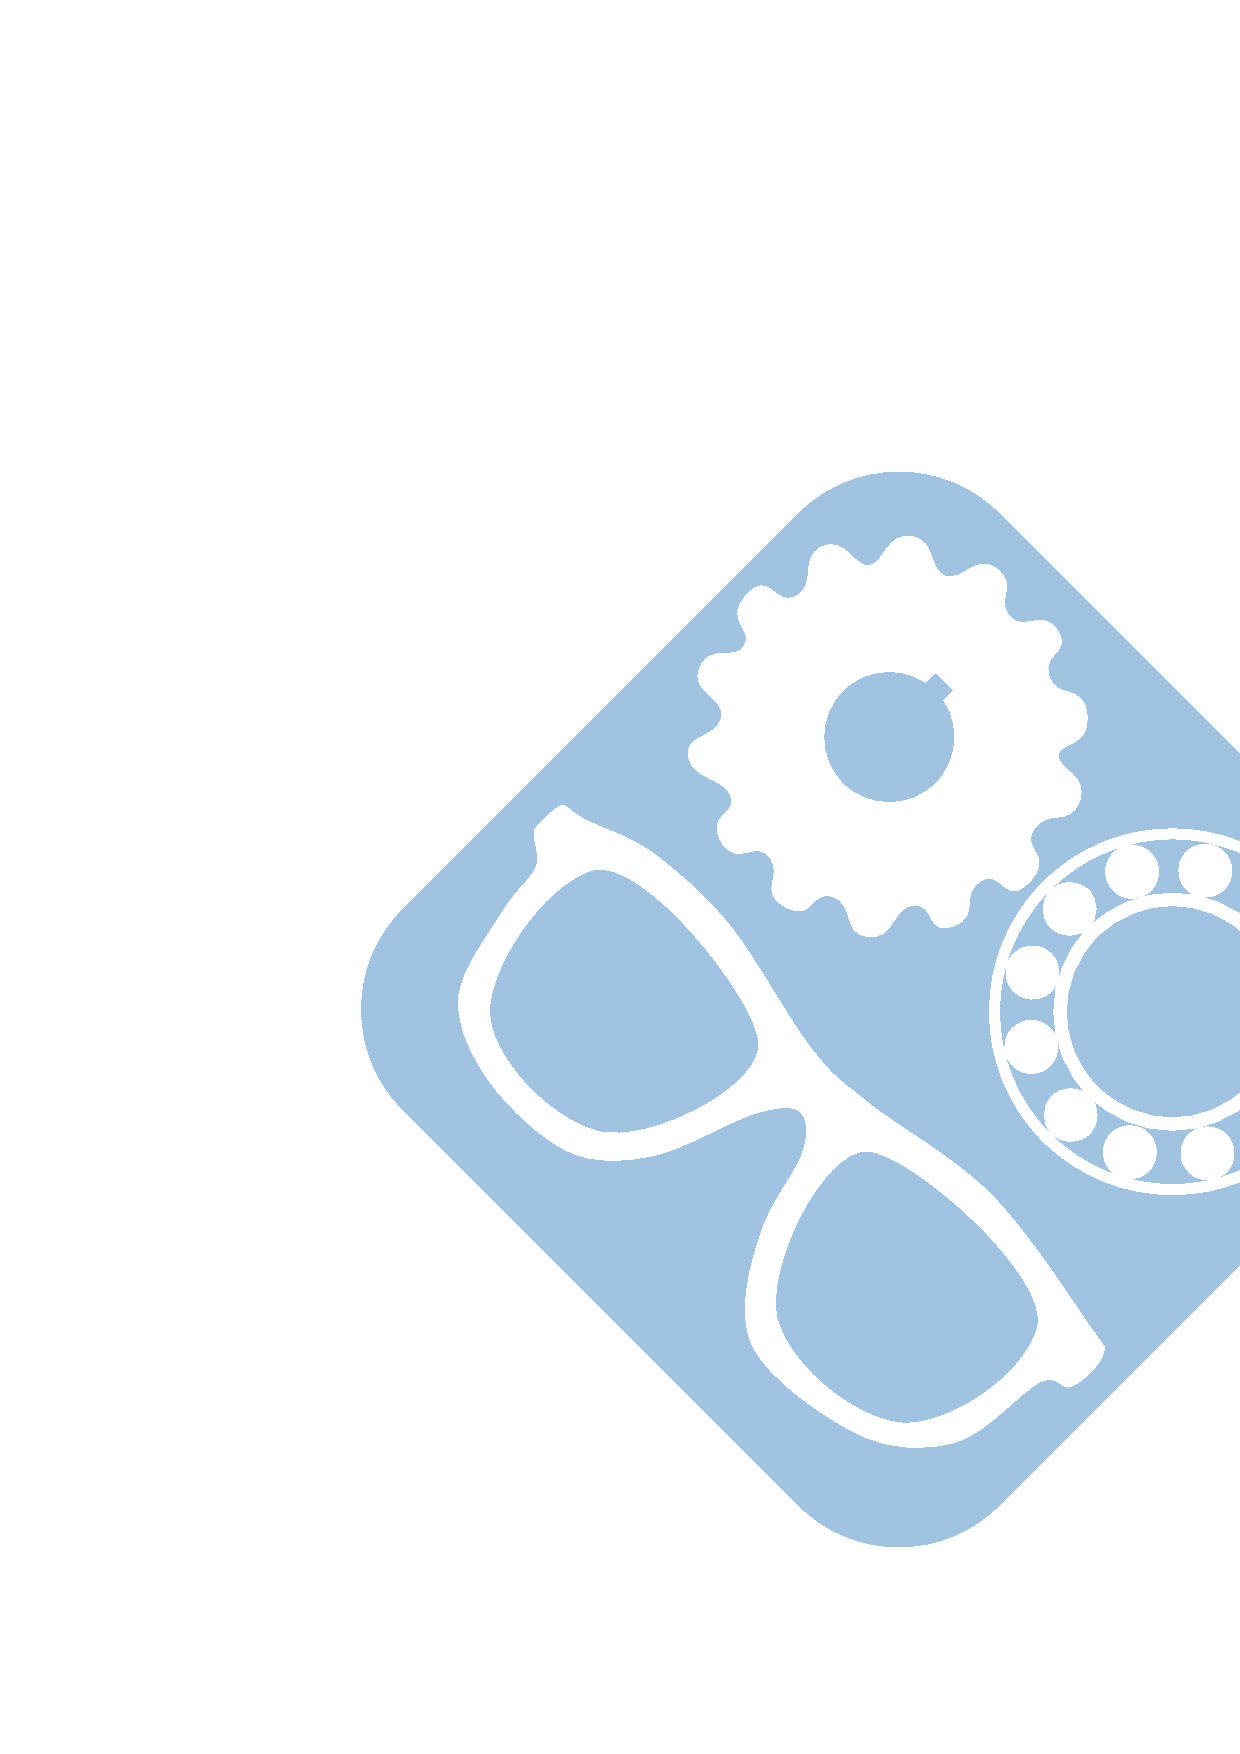
\includegraphics[width=\paperwidth,height=\paperheight,%
keepaspectratio]{../../img/fond3}%
\end{center}
\vfill
}}}

\newcommand{\BackgroundPicdeux}{%
\put(25,-30){%
\parbox[b][\paperheight]{\paperwidth}{%
\vfill
\begin{center}
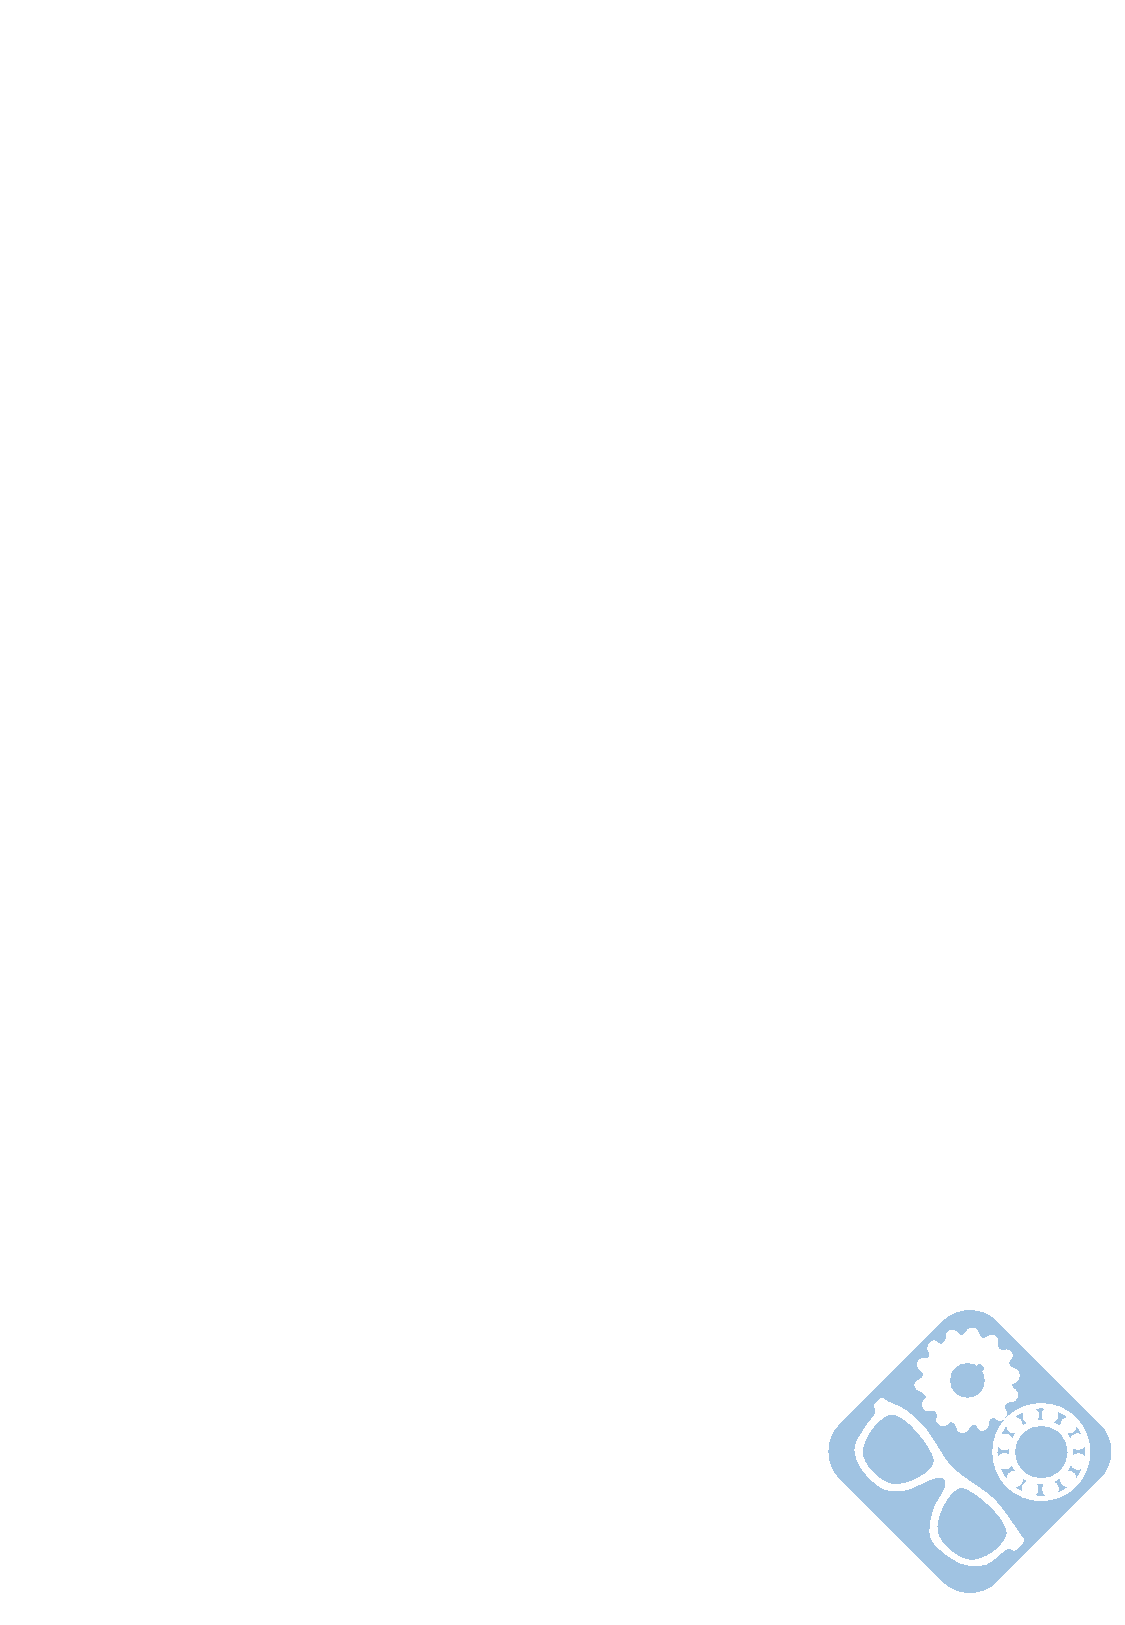
\includegraphics[width=\paperwidth,height=\paperheight,%
keepaspectratio]{../../img/fond4}%
\end{center}
\vfill
}}}

\begin{document}

\pagestyle{empty}

\AddToShipoutPicture*{\BackgroundPic}


\includegraphics[width=2cm]{../../img/logo}

\Huge{DS \num\ - \sujet}

\vspace{1cm}

\ifdef{\prive}{\begin{center}\colorbox{danger}{\Huge{Avec Correction}}\end{center}}{}

\begin{center}
\centering\huge{PTSI}
\end{center}

\vspace{2cm}


\begin{center}
\centering\Large{\jour}
\end{center}

\vspace{2cm}

\normalsize

\tableofcontents

\newpage

\AddToShipoutPicture{\BackgroundPicdeux}

\pagestyle{fancy}

\begin{center}
\Huge \sujet
\end{center}


\normalsize

\section{Présentation du système}

Il est aujourd'hui possible de réduire les temps de parcours en train grâce à la grande vitesse. Malheureusement, cette technologie nécessite la construction d'un réseau ferré spécifique et coûteux : les lignes à grande vitesse.

Sur ligne classique, une augmentation de la vitesse du train conduirait à une dégradation du confort du passager en particulier lors du passage en courbe.

En courbe, le passager est soumis à une accélération transversale (accélération centripète) qui au-delà d'une certaine valeur devient gênante, inconfortable. Pour compenser cette accélération transversale, la voie est posée avec un dévers dans les portions de courbe, c'est-à-dire que le plan des rails est incliné par rapport au plan horizontal (le rail extérieur est plus haut que le rail intérieur).

\begin{figure}[!h]
 \centering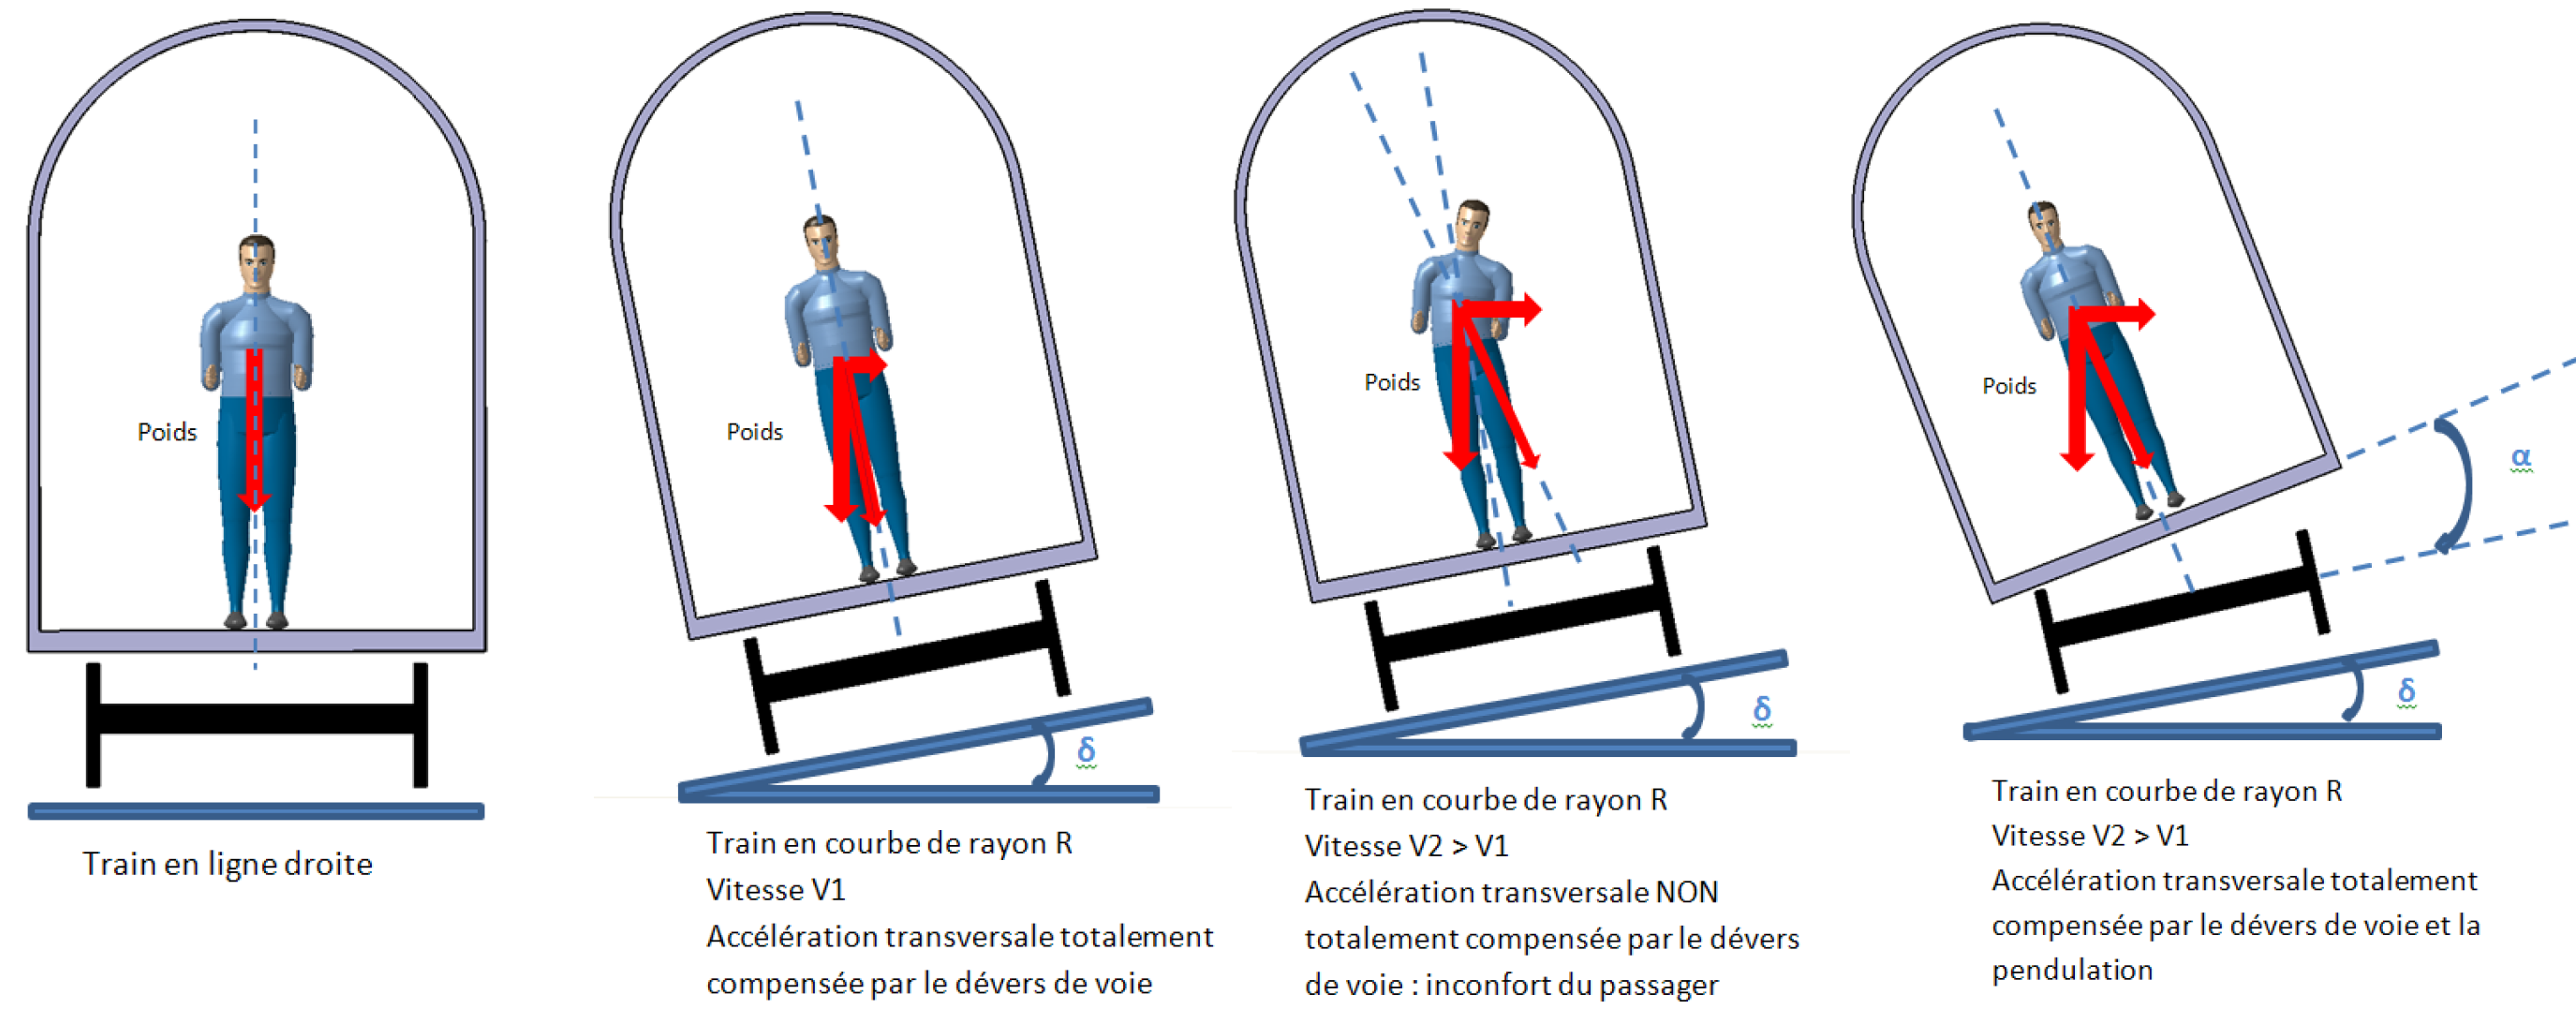
\includegraphics[width=\linewidth]{img/fig1}
 \caption{Comparaison train classique et pendulaire en courbe}
 \label{img01}
\end{figure}

Une alternative moins coûteuse que le TGV est possible avec le train pendulaire.

La pendulation est un moyen efficace pour l'amélioration du confort des passagers et la réduction sensible des temps de parcours (de 15 à 25\%) et ce, en circulation sur voie classique, donc avec un minimum d'impact sur les infrastructures.

Elle autorise, par inclinaison de la caisse autour de son axe longitudinal (angle d'inclinaison qui s'ajoute à l'angle de dévers) la diminution de l'accélération transversale ressentie par les passagers et permet ainsi un passage en courbe à une vitesse plus importante qu'un train classique pour le même niveau de confort.

L'étude proposée ici porte sur le système de pendulation de train interposé entre le bogie et la caisse.

Ce système est composé de deux actionneurs (ou vérins) montés en opposition. Pendant que l'un des actionneurs \og pousse \fg la caisse l'autre « tire ».

Ces actionneurs inclinent la caisse en agissant sur une traverse qui supporte celle-ci.

La traverse est \og suspendue \fg au bogie grâce à 4 bielles montées en liaisons pivot. Ce système de bielles permet d'obtenir la cinématique de pendulation.

Ce dispositif installé sous la suspension secondaire permet de garantir une excellente stabilité du bogie.

Le mécanisme de pendulation étant situé au-dessous des suspensions secondaires, le comportement des suspensions reste inchangé par rapport à un bogie conventionnel.

\begin{figure}[!h]
 \centering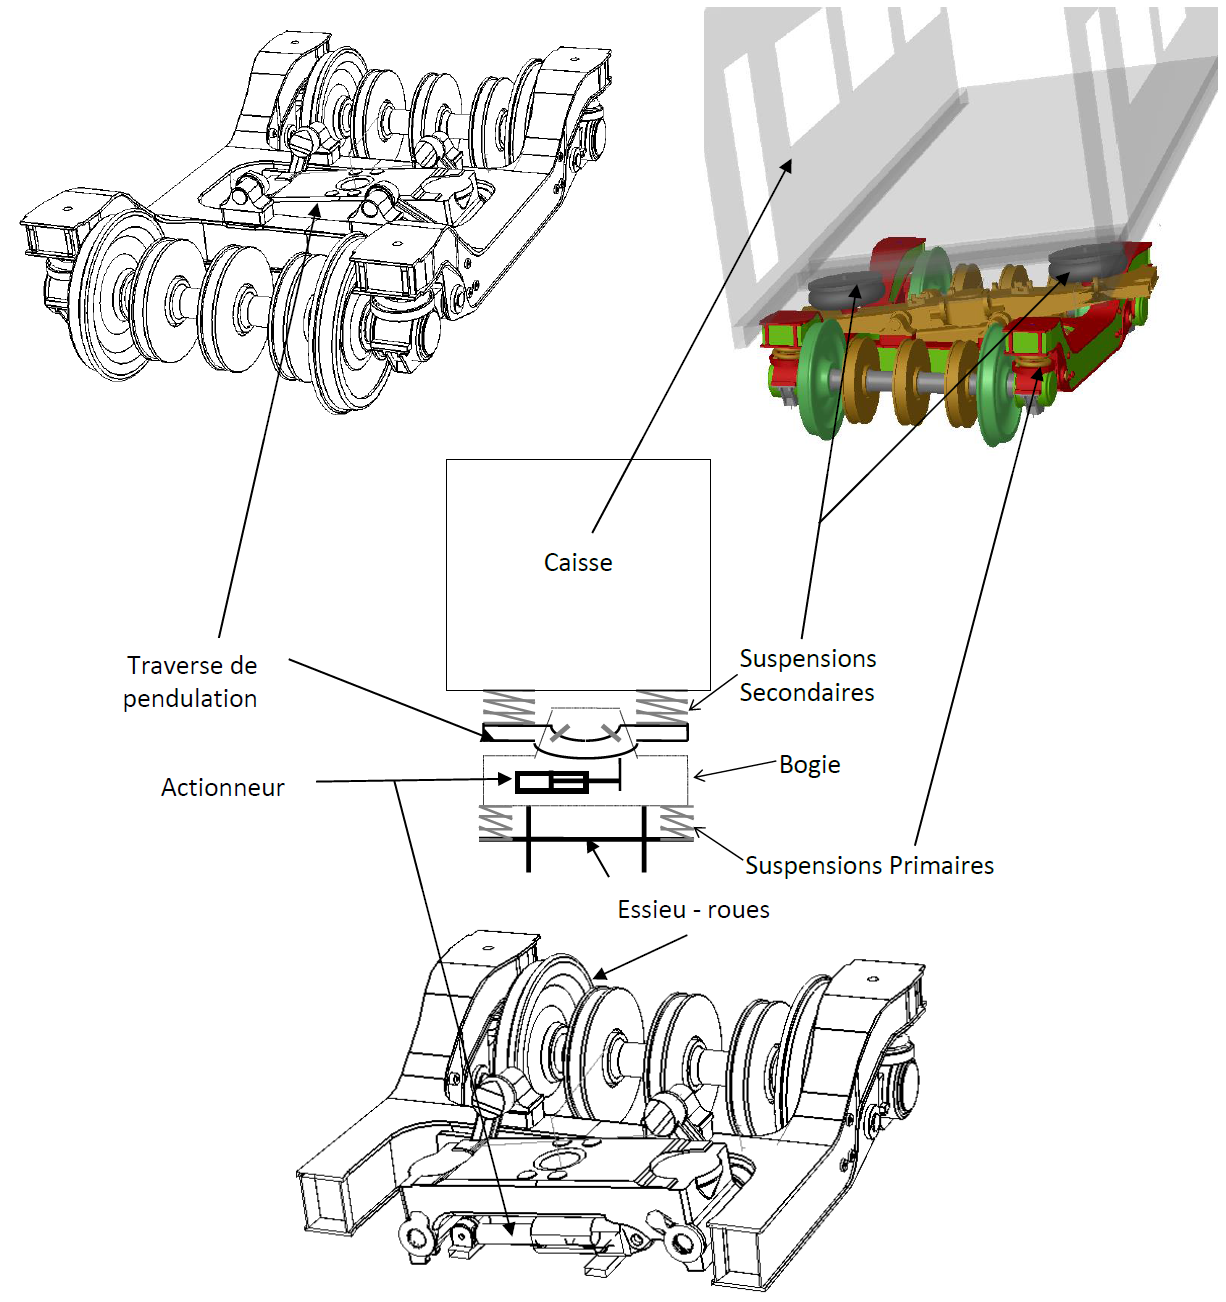
\includegraphics[width=0.65\linewidth]{img/fig2}
 \caption{Schéma du système de pendulation}
 \label{img02}
\end{figure}

\subsection{Problématique et objectifs de l'étude}

Les trains pendulaires actuellement en service fonctionnent à l'aide d'actionneurs électro-hydrauliques. Cette technologie conduit à des coûts de maintenance très importants. Les concepteurs ont donc étudié la faisabilité d'une pendulation avec actionneurs électromécaniques.

Le système d'actionnement électromécanique présente de nombreux avantages par rapport à la solution électro-hydraulique :
\begin{itemize}
 \item fiabilité accrue,
 \item maintenance moins coûteuse,
 \item poids inférieur,
 \item encombrement réduit,
 \item consommation en énergie plus faible.
\end{itemize}

Ces actionneurs sont plus chers à l'achat mais le coût global de possession de ce système le rend avantageux.

\paragraph{Objectif:}
L'objectif général de l'étude est de modéliser le système de pendulation afin de vérifier la faisabilité d'une technologie de pendulation électromécanique et d'en dimensionner les principaux composants mécaniques, électriques et de commande.

\subsection{Fonctions et diagrammes SysMl}

\begin{figure}[!h]
 \centering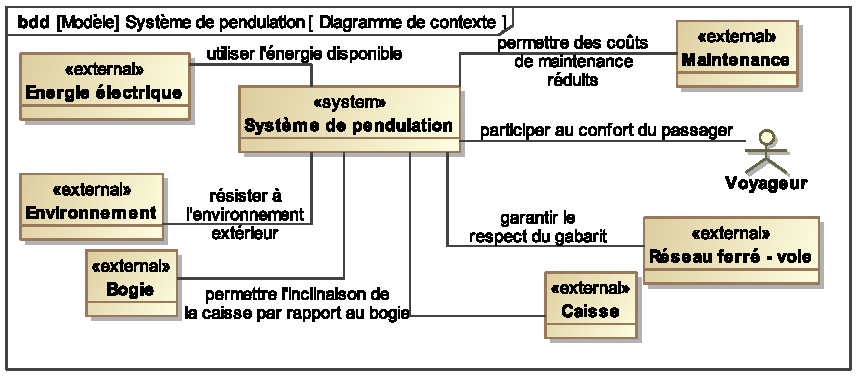
\includegraphics[width=0.9\linewidth]{img/diagramme_contexte}
 \caption{Diagramme de contexte}
 \label{contexte}
\end{figure}

\begin{table}[!h]
\begin{tabular}{|l|l|}
\hline
Critère & Niveau \\
\hline
Masse de l'ensemble caisse + traverse(par bogie) & $Mc=35tonnes$ \\
Angle de pendulation maximal entre traverse et bogie & $\alpha_{max}=\pm6,3\degree$ \\
\hline
Accélération non compensée maximale & $\gamma_{ncmax}=1,2m.s^{-2}$ \\
\hline
\end{tabular}
 \caption{Caractéristiques du système}
 \label{caracteristiques}
\end{table}

\begin{figure}[!h]
 \centering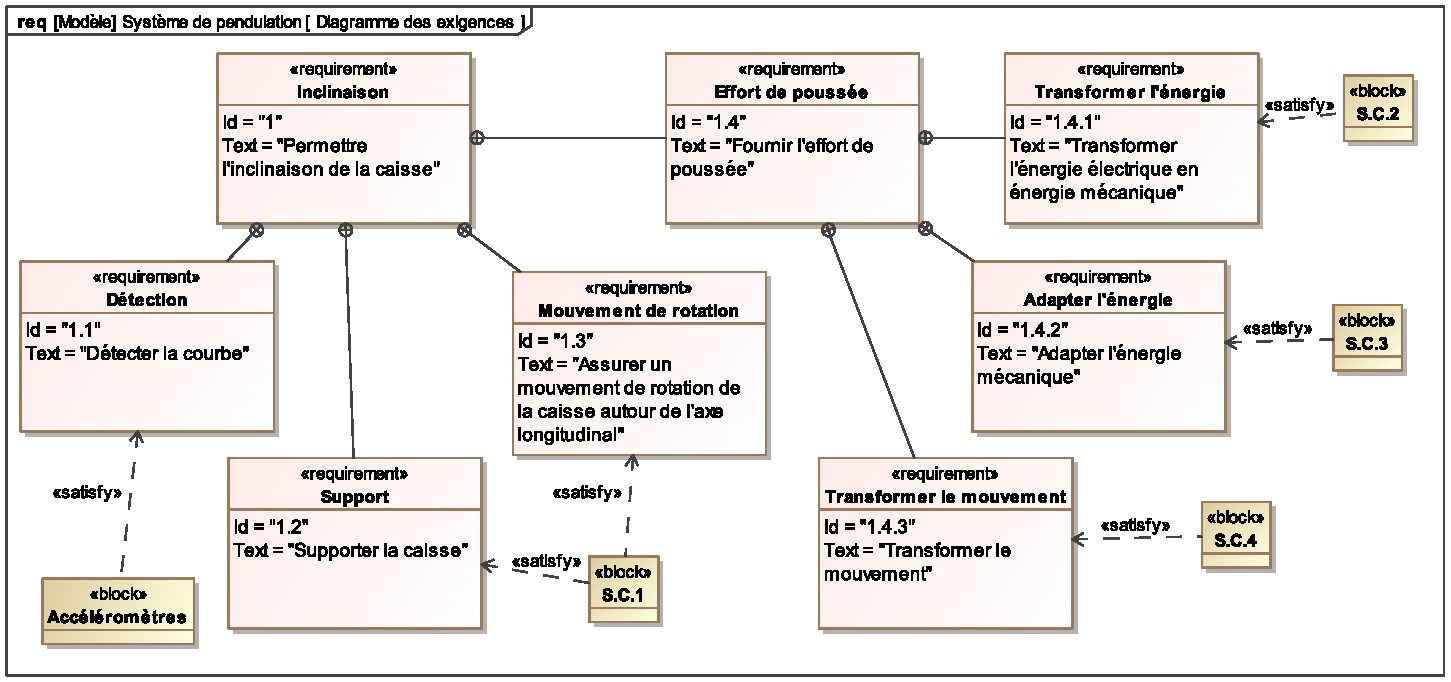
\includegraphics[width=\linewidth]{img/diagramme_exigences}
 \caption{Diagramme d'exigences}
 \label{exigences}
\end{figure}

\newpage

\section{Analyse fonctionnelle et structurelle}

~\

\begin{figure}[!h]
 \centering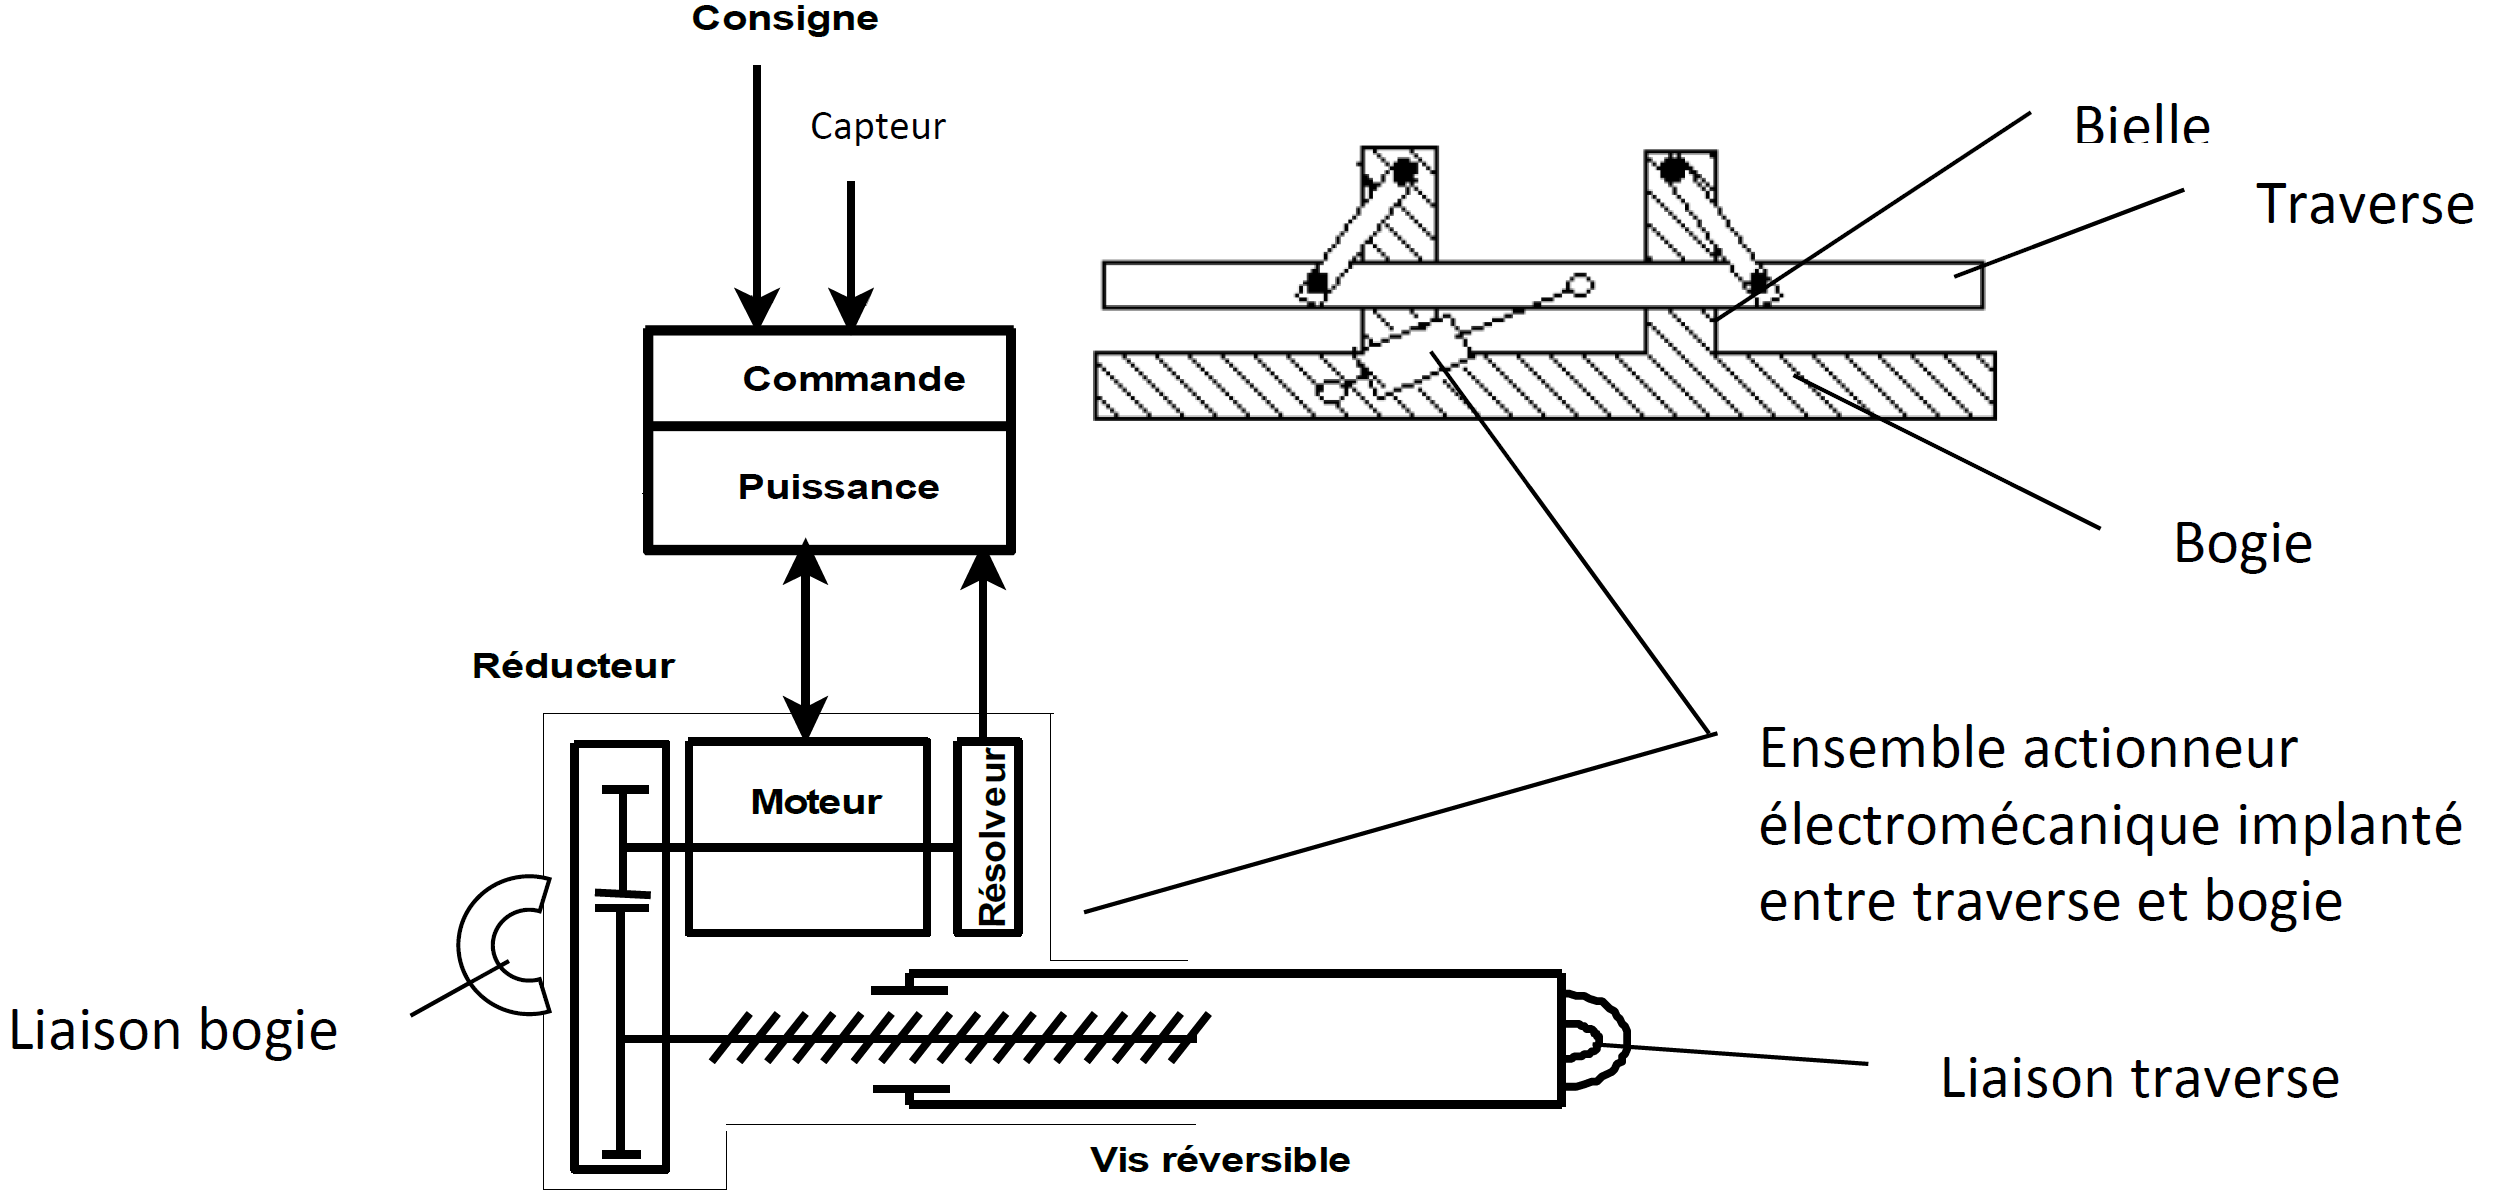
\includegraphics[width=0.7\linewidth]{img/fig3}
 \caption{Schéma de principe commande, actionneur, traverse de pendulation}
 \label{img03}
\end{figure}

\question{À l'aide du schéma de principe figure \ref{img03} et de la présentation du système fournis au
premier paragraphe, indiquer sur le document réponse quelles sont les solutions
constructives (S.C.1 à S.C.4) choisies par le constructeur pour assurer la réalisation des fonctions techniques.}

\begin{figure}[!h]
 \centering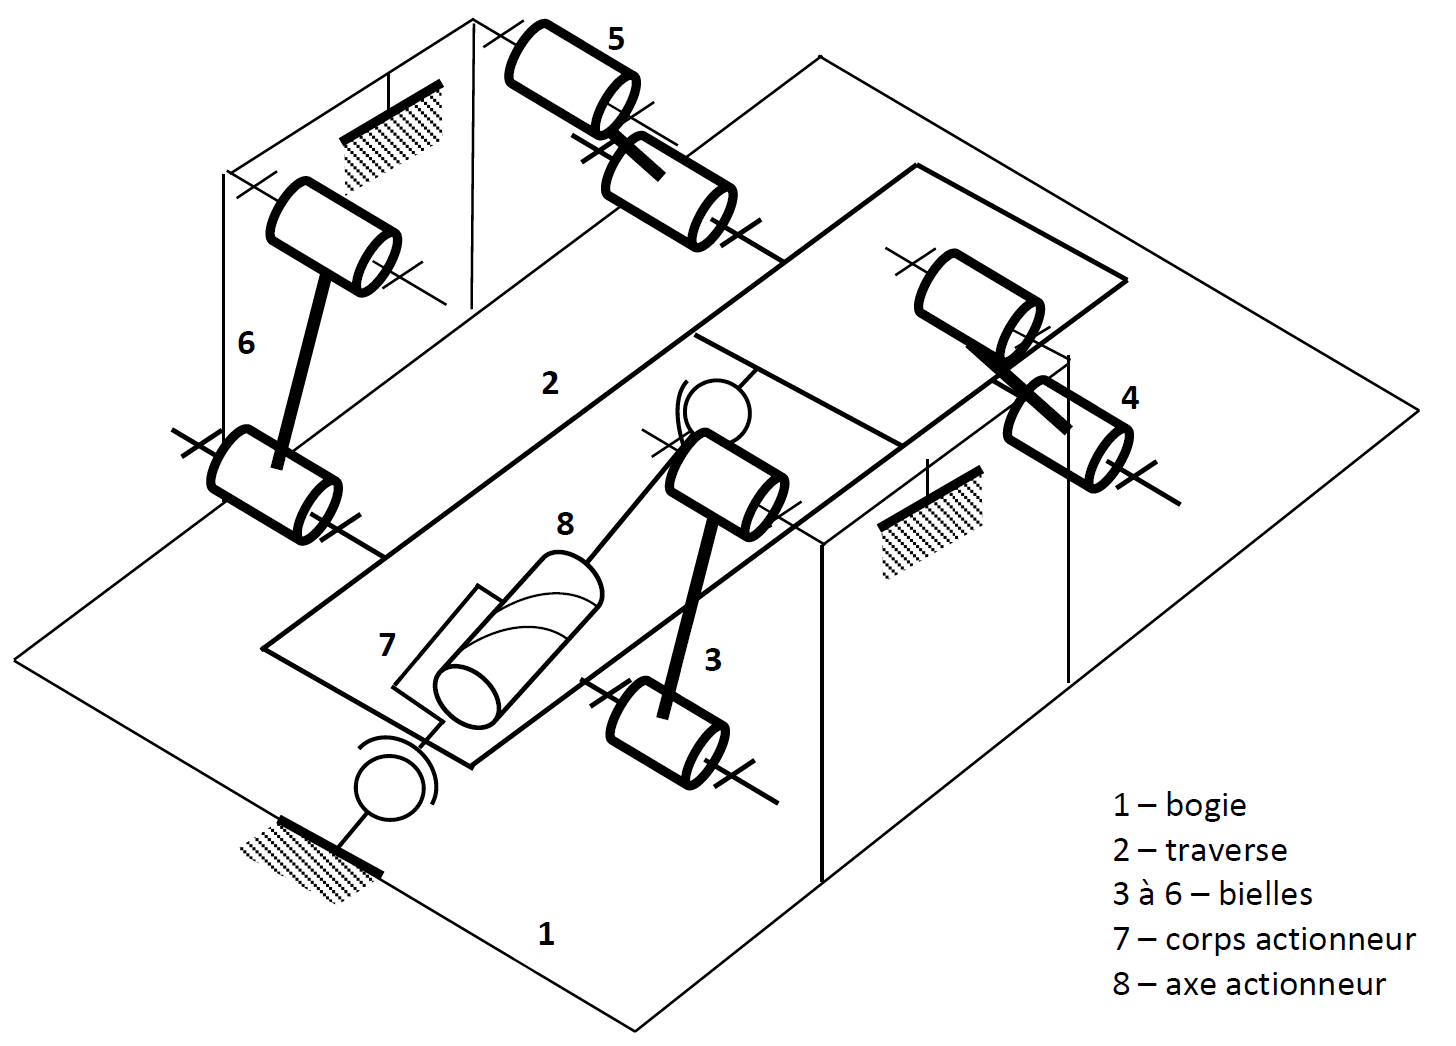
\includegraphics[width=0.7\linewidth]{img/fig4}
 \caption{Schéma cinématique ensemble de pendulation (un seul actionneur représenté)}
 \label{img04}
\end{figure}

\question{Sur le document réponse, à l'aide du schéma cinématique fourni figure \ref{img04} compléter le graphe de liaisons en indiquant pour chaque liaison leur nom et nombre d'inconnues statiques. Déterminer le degré d'hyperstatisme de l'ensemble.}

~\

On supposera l'actionneur électromécanique modélisable par un axe en liaison hélicoïdale avec le corps de l'actionneur. Sur la figure \ref{img04}, un seul actionneur est modélisé.

Du fait de la symétrie du problème il est possible de réaliser une étude simplifiée de la cinématique de pendulation en ne modélisant qu'un seul actionneur, la traverse et deux bielles, le tout étant ramené dans le plan.

\question{Sur le document réponse compléter le schéma cinématique dans le plan du système de pendulation. Déterminer le degré d'hyperstatisme de l'ensemble pour le modèle plan.}

\question{A partir des résultats obtenus aux questions Q2 et Q3, conclure quant aux principales contraintes géométriques qui seraient à spécifier sur le système complet pour assurer un montage et fonctionnement correct du système.}

\section{Étude de la fonction \og diminuer les temps de parcours d'au moins 15\% \fg}

L'objectif de cette étude est d'évaluer, pour un angle de pendulation maximal imposé par le respect du gabarit, la compensation de dévers obtenue et en déduire le gain de vitesse possible dans une courbe de référence fournie en figure \ref{img05} ci-dessous.

\begin{figure}[!h]
 \centering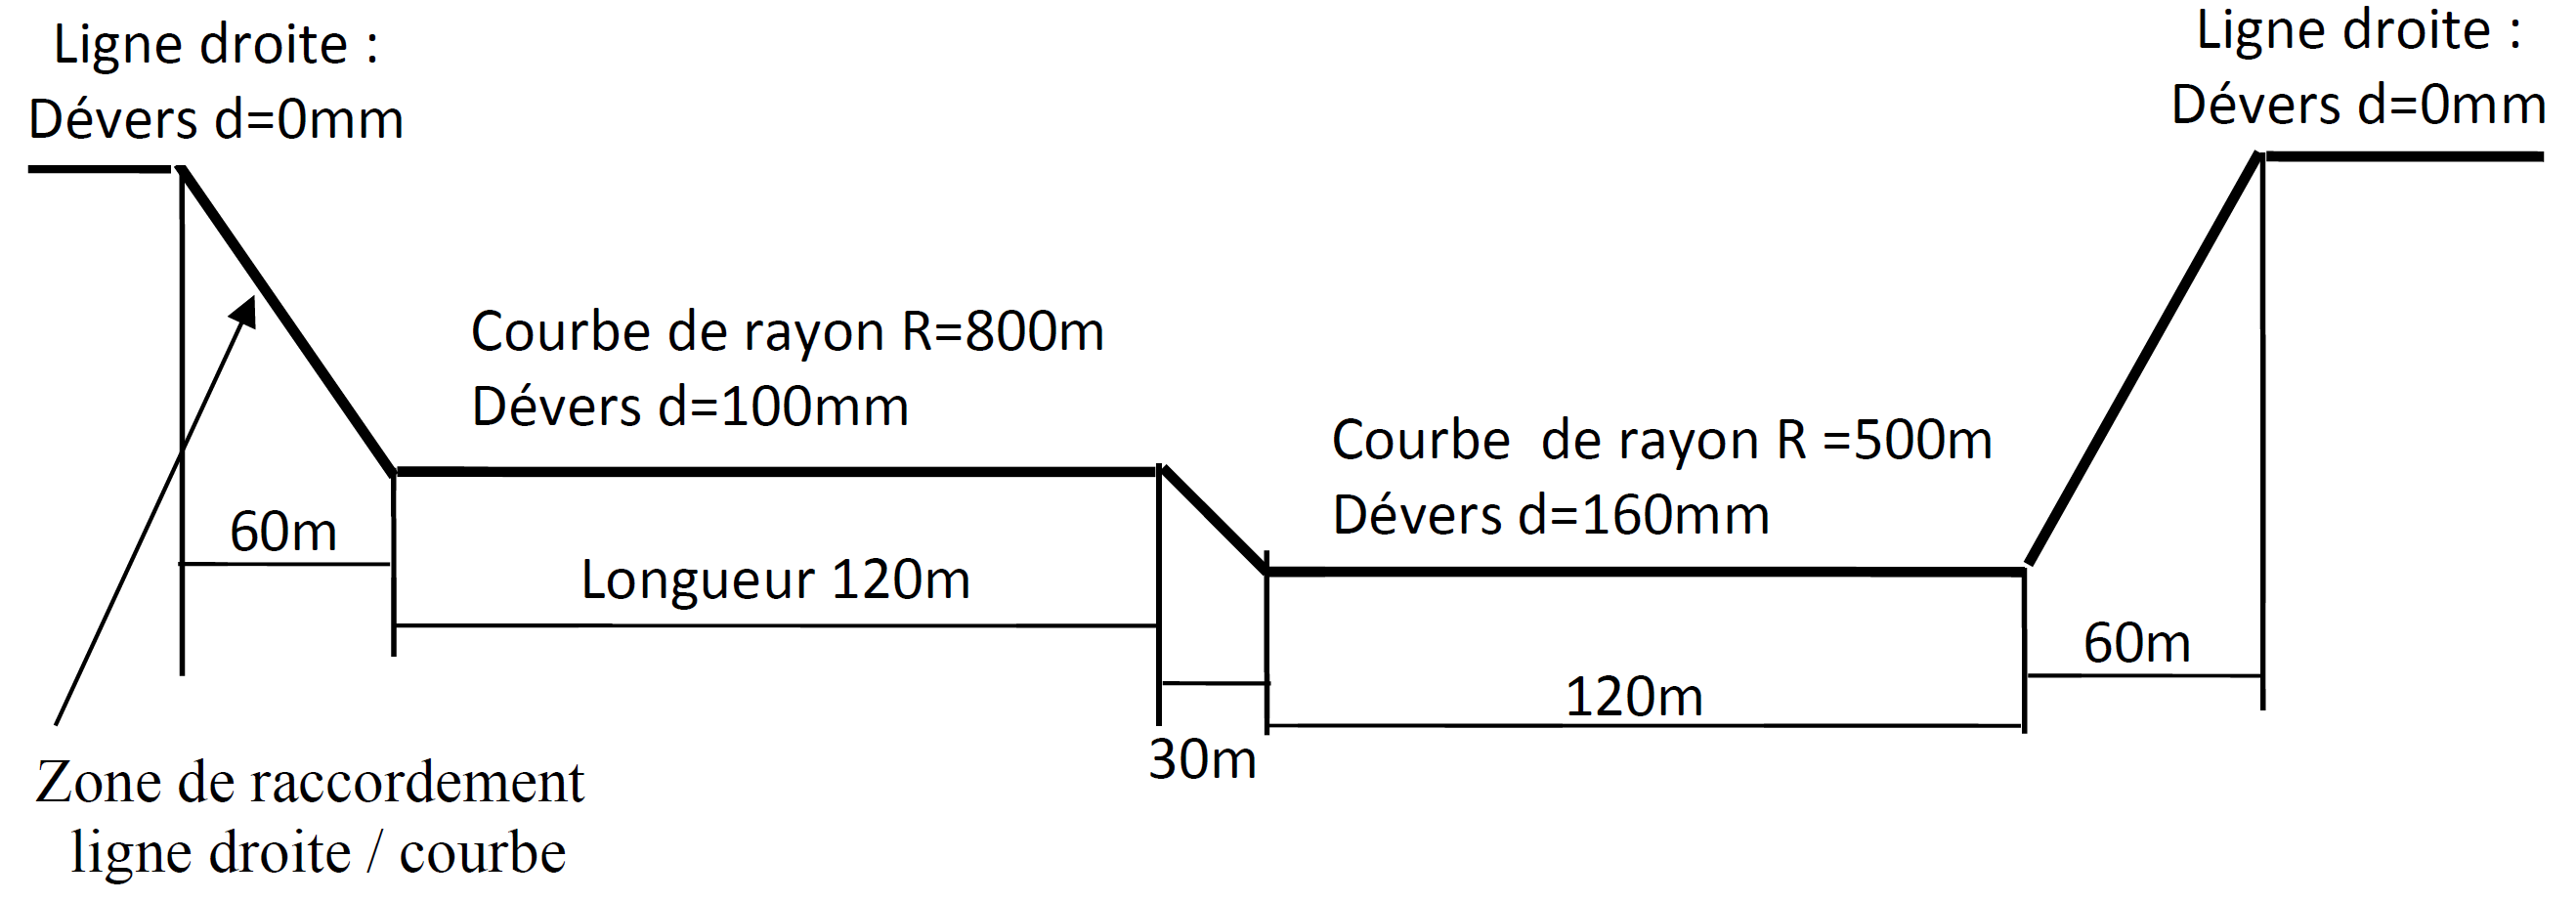
\includegraphics[width=0.7\linewidth]{img/fig5}
 \caption{Tracé de voie : courbe de référence}
 \label{img05}
\end{figure}

\textbf{Hypothèses et notations (cf figure \ref{img06}) :}
Dans un premier temps, le véhicule est considéré classique sans système de pendulation :
\begin{itemize}
 \item l'ensemble $\{D\}$ constitué de la caisse, du bogie et des essieux est supposé indéformable,
 \item les liaisons sont supposées parfaites,
 \item l'écartement des rails est noté $e$,
 \item l'angle de dévers de pose de la voie est noté $\delta$,
 \item le dévers de voie en mm est noté $d$,
 \item le point G est le centre de gravité de l'ensemble $\{D\}$.
\end{itemize}

\newpage

\begin{figure}[!h]
 \centering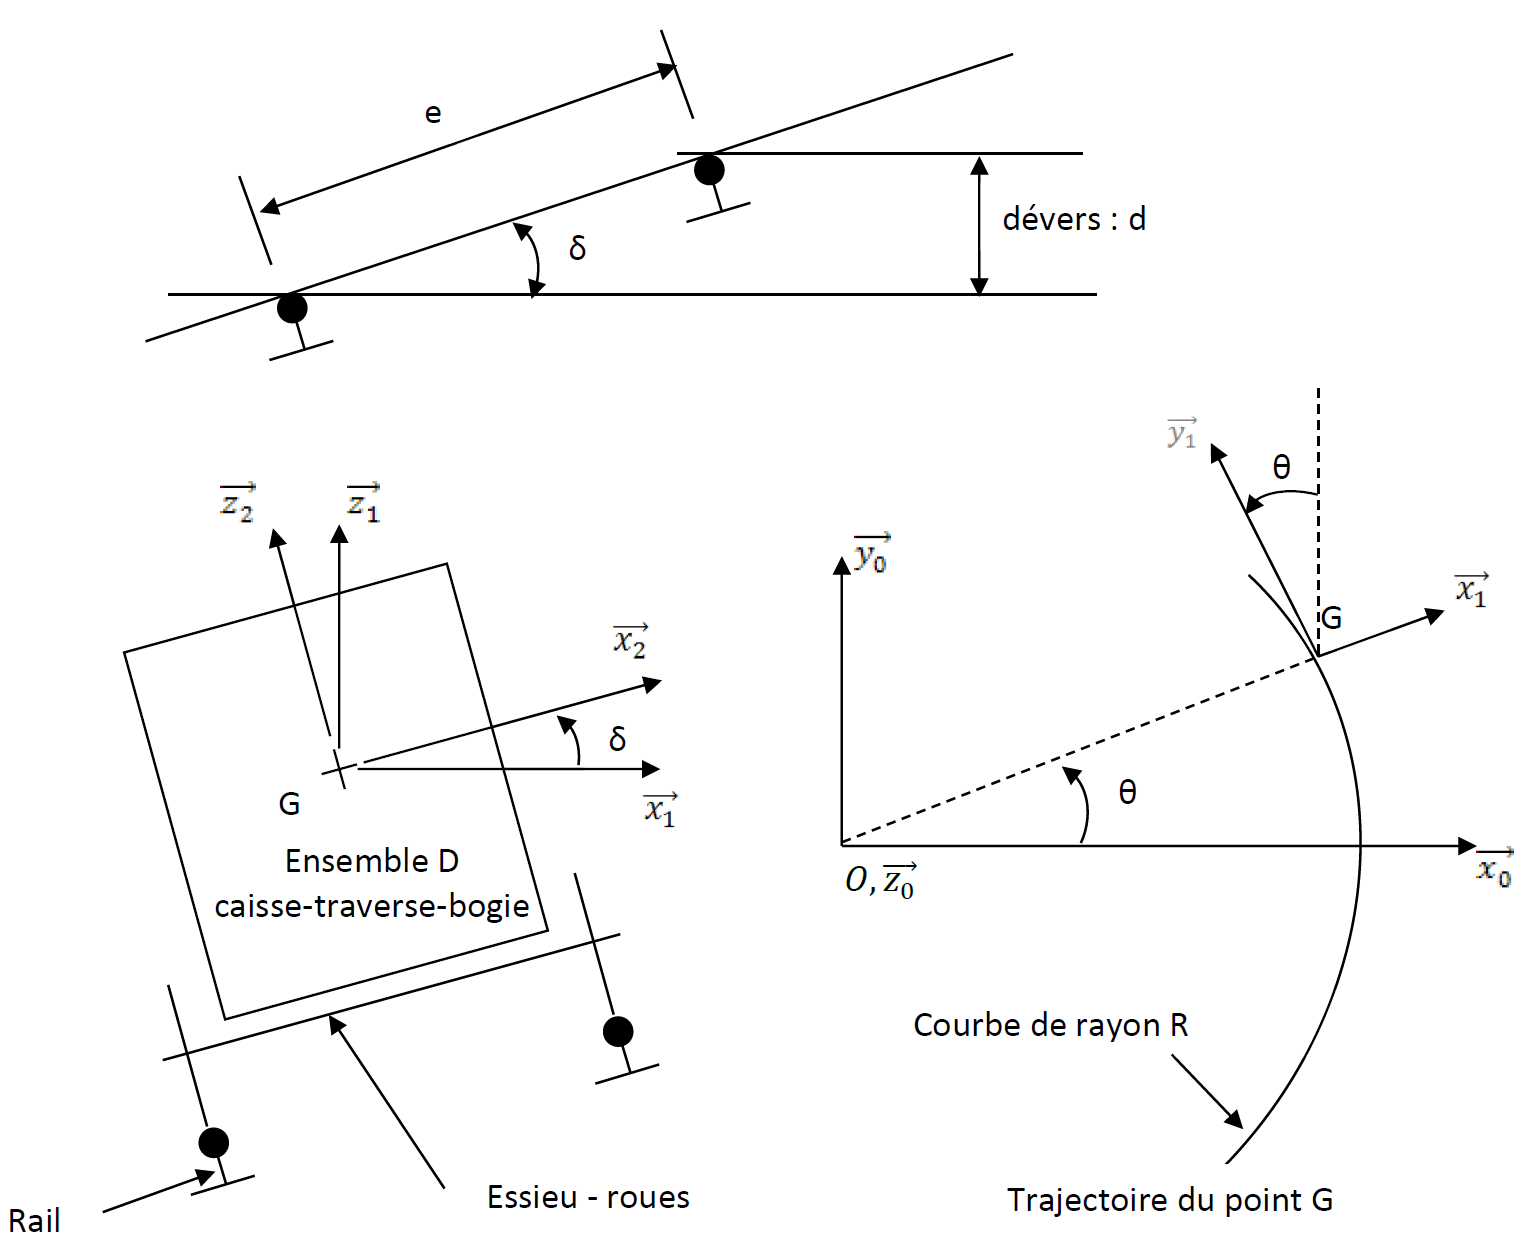
\includegraphics[width=0.7\linewidth]{img/fig6}
 \caption{Modélisation de la voie}
 \label{img06}
\end{figure}

Soit $R_0(O,\overrightarrow{x_0},\overrightarrow{y_0},\overrightarrow{z_0})$ repère de référence supposé Galiléen.

L'axe $(O,\overrightarrow{z_0})$ est perpendiculaire au plan de la trajectoire du véhicule.

L'accélération de la pesanteur est désignée par $\overrightarrow{g}=-g.\overrightarrow{z_0}$.

Le repère $R_1(O,\overrightarrow{x_1},\overrightarrow{y_1},\overrightarrow{z_1})$ suit le point G dans son mouvement curviligne (courbe de rayon R et de centre O).

La vitesse d'avance du véhicule est supposée constante avec $\overrightarrow{V_{G\in R_1/R_0}}=V.\overrightarrow{y_1}$.

L'angle $\delta$ est très faible ce qui permet l'approximation suivante : $cos \delta = 1$.

\question{Exprimer l'accélération $\overrightarrow{a_{G/R0}}$ du point G par rapport à $R_0$ en fonction de V et R.}

Soit $\gamma_{nc}$ la composante d'accélération appelée accélération non compensée. Elle correspond à l'accélération latérale équivalente réellement ressentie par le passager.

\question{Montrer que $\gamma_{nc}=(\vec{g}-\overrightarrow{a_{G/R0}}).\overrightarrow{x_2}$ peut s'écrire sous la forme : $\gamma_{nc}=\frac{V^2}{R}-g.\frac{d}{e}$.}

\question{Exprimer en fonction de V, R, g et e, l'angle de dévers $\delta$ puis le dévers de voie d permettant d'annuler cette composante $\gamma_{nc}$.}

Application numérique :
\begin{itemize}
 \item rayon de courbe $R=800m$,
 \item dévers de voie installé : $d=100mm$,
 \item vitesse du véhicule $V=145km.h^{-1}$,
 \item écartement de voie $e=1150mm$,
 \item $g=10m.s^{-2}$.
\end{itemize}

\question{Calculer la composante d'accélération non compensée $\gamma_{nc}$.}

\question{Représenter sur la figure du document réponse les différents vecteurs $\vec{g}$, $-\overrightarrow{a_{G/R0}}$ et $\gamma_{nc}.\overrightarrow{x_2}$.}

L'insuffisance de dévers correspond à ce qu'il faudrait ajouter au dévers de voie installé pour annuler l'accélération non compensée $\gamma_{nc}$.

\question{Calculer l'insuffisance de dévers puis l'angle de dévers correspondant exprimé en degré.}

~\

On prendra pour la suite $sin(\delta+\alpha)\simeq0,31$.

\paragraph{On s'intéresse maintenant au véhicule équipé du système de pendulation de caisse.}

~\

\begin{figure}[!h]
 \centering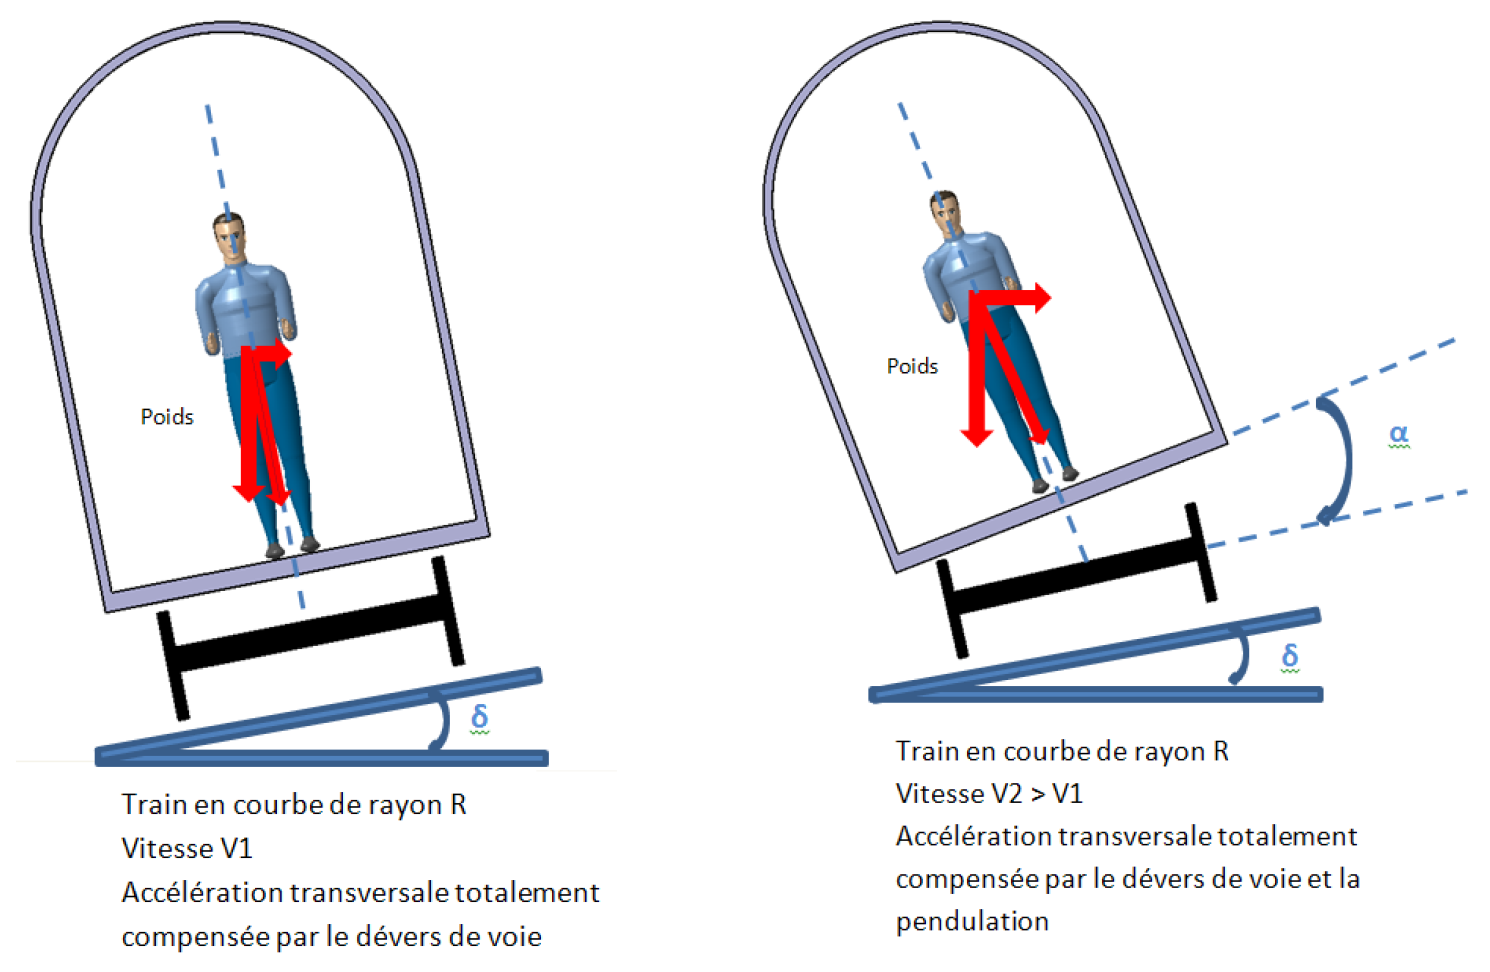
\includegraphics[width=0.8\linewidth]{img/fig6_b}
 \label{img06_b}
\end{figure}

Les normes ferroviaires imposent que l'accélération latérale en courbe ressentie par un passager (accélération latérale non compensée) ne dépasse pas 1,2 .

L'angle de pendulation de caisse est noté $\alpha$.

L'inclinaison de la caisse $\alpha$ obtenue grâce au système de pendulation permet de compenser le manque de dévers de voie pour augmenter la vitesse en courbe tout en limitant l'accélération non compensée.

Le respect du gabarit du train autorise une inclinaison maximale de la caisse par rapport au plan des rails de $\alpha_{MAX}=6,3\degree$. Cette inclinaison vient s'ajouter à l'angle de dévers de voie $\delta$.

\question{Déterminer la vitesse que pourra atteindre le véhicule dans cette courbe de référence en respectant l'accélération non compensée maximale autorisée.}

\question{Conclure vis-à-vis des gains de temps espérés.}

\section{Étude de la \og assurer un mouvement de rotation de la caisse \fg}

L'objectif de cette étude est de caractériser la course et la vitesse de sortie d'axe d'actionneur vis-à-vis des objectifs de rapidité de pendulation. Ces caractéristiques permettront la validation du choix préliminaire de l'actionneur électro-mécanique par le concepteur.

L'épure suivante représente le système de pendulation ramené dans le plan, pour un angle de dévers $\delta$ de 5° et un angle quelconque d'inclinaison de caisse.

\begin{figure}[!h]
 \centering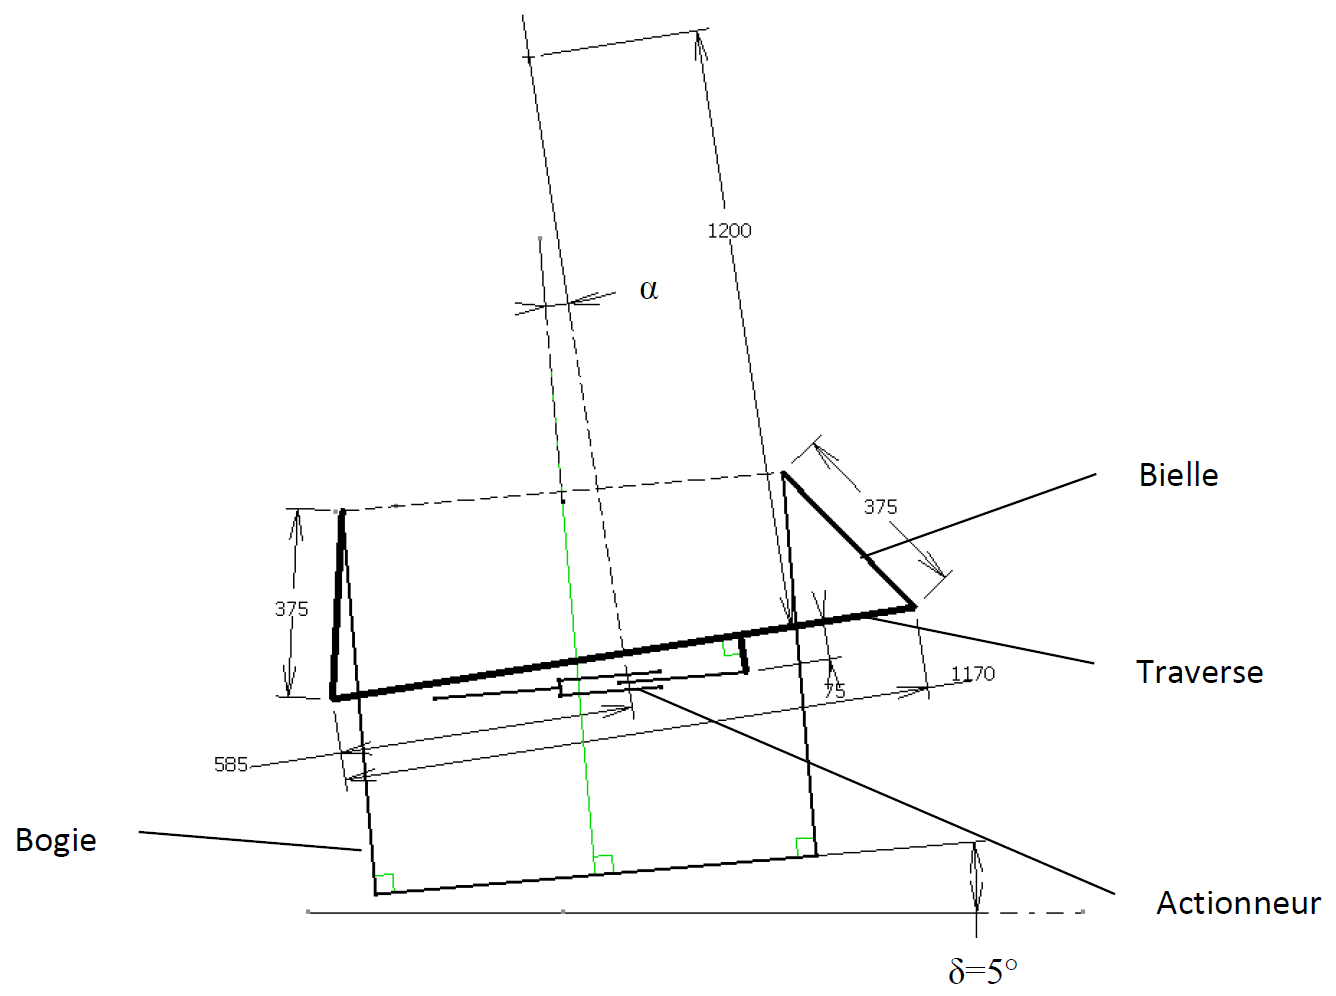
\includegraphics[width=0.7\linewidth]{img/fig10}
  \caption{Epure du système de pendulation ramené dans le plan}
 \label{img10}
\end{figure}

On donne une vitesse de rotation à imposer à la caisse de $0,1rad.s^{-1}$.

\question{Sur le document réponse représentant le système pour une pendulation de caisse intermédiaire $\alpha$ de 5° et un angle de dévers $\delta$ de 5° :
\begin{itemize}
 \item tracer le support de la vitesse du point B de la traverse pendulaire : $\overrightarrow{V_{B\in2/1}}$ en mouvement par rapport au châssis de bogie. Justifier.
 \item tracer le support de la vitesse du point D de la traverse pendulaire : $\overrightarrow{V_{D\in2/1}}$ en mouvement par rapport au châssis de bogie.
 \item placer alors sur le dessin le point $I_{21}$ Centre Instantané de rotation du mouvement de 2 par rapport à 1.
 \item tracer le support de la vitesse du point H, $\overrightarrow{V_{H\in2/1}}$ de la traverse en mouvement par rapport au châssis.
 \item pour la vitesse de rotation de caisse fournie, en déduire graphiquement l'amplitude de la vitesse de sortie d'axe d'actionneur $\|\overrightarrow{V_{D\in2/1}}\|$.
\end{itemize}}

La vitesse d'axe d'actionneur suit la loi trapézoïdale suivante :

\begin{figure}[!h]
 \centering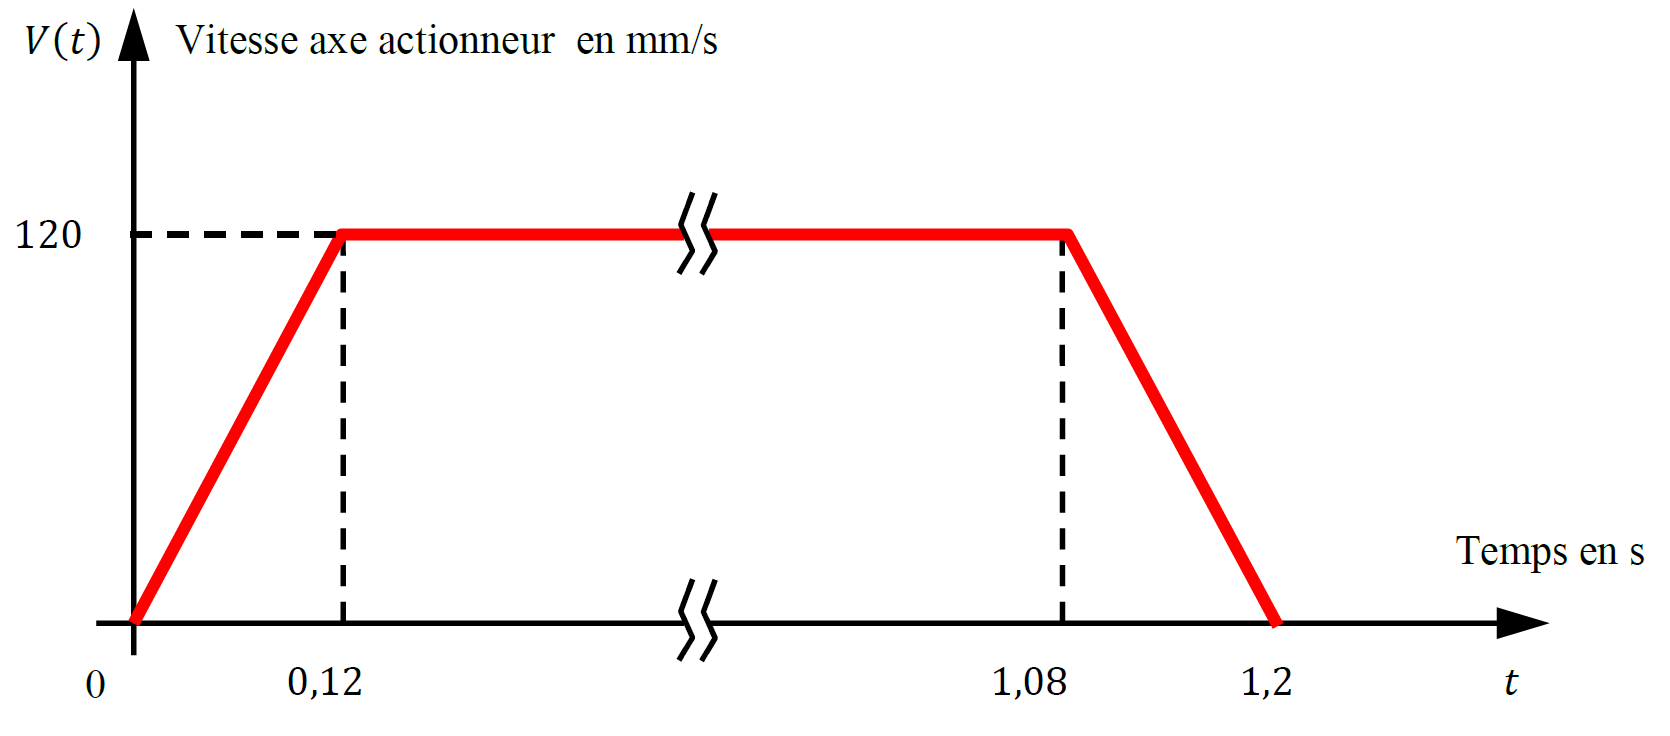
\includegraphics[width=0.6\linewidth]{img/fig11}
 \caption{Loi de vitesse axe actionneur pour un angle $\alpha$ = 6,3°}
 \label{img11}
\end{figure}

L'accélération imposée à l'axe de l'actionneur est au maximum de 1 $m.s^{-2}$.

\question{Déterminer la course de l'actionneur $X_v(t)$ au cours du temps.}

\question{En déduire la course totale nécessaire pour atteindre un angle de pendulation de 6,3°.}

\section{Modélisation de l'asservissement du système.}

Les réponses Q16 à Q22 sont à reporter sur le document réponse.

L'objectif de cette partie est d'étudier l'asservissement en position de l'ensemble {traverse+caisse} décrit figure \ref{img15}.

\begin{figure}[!h]
 \centering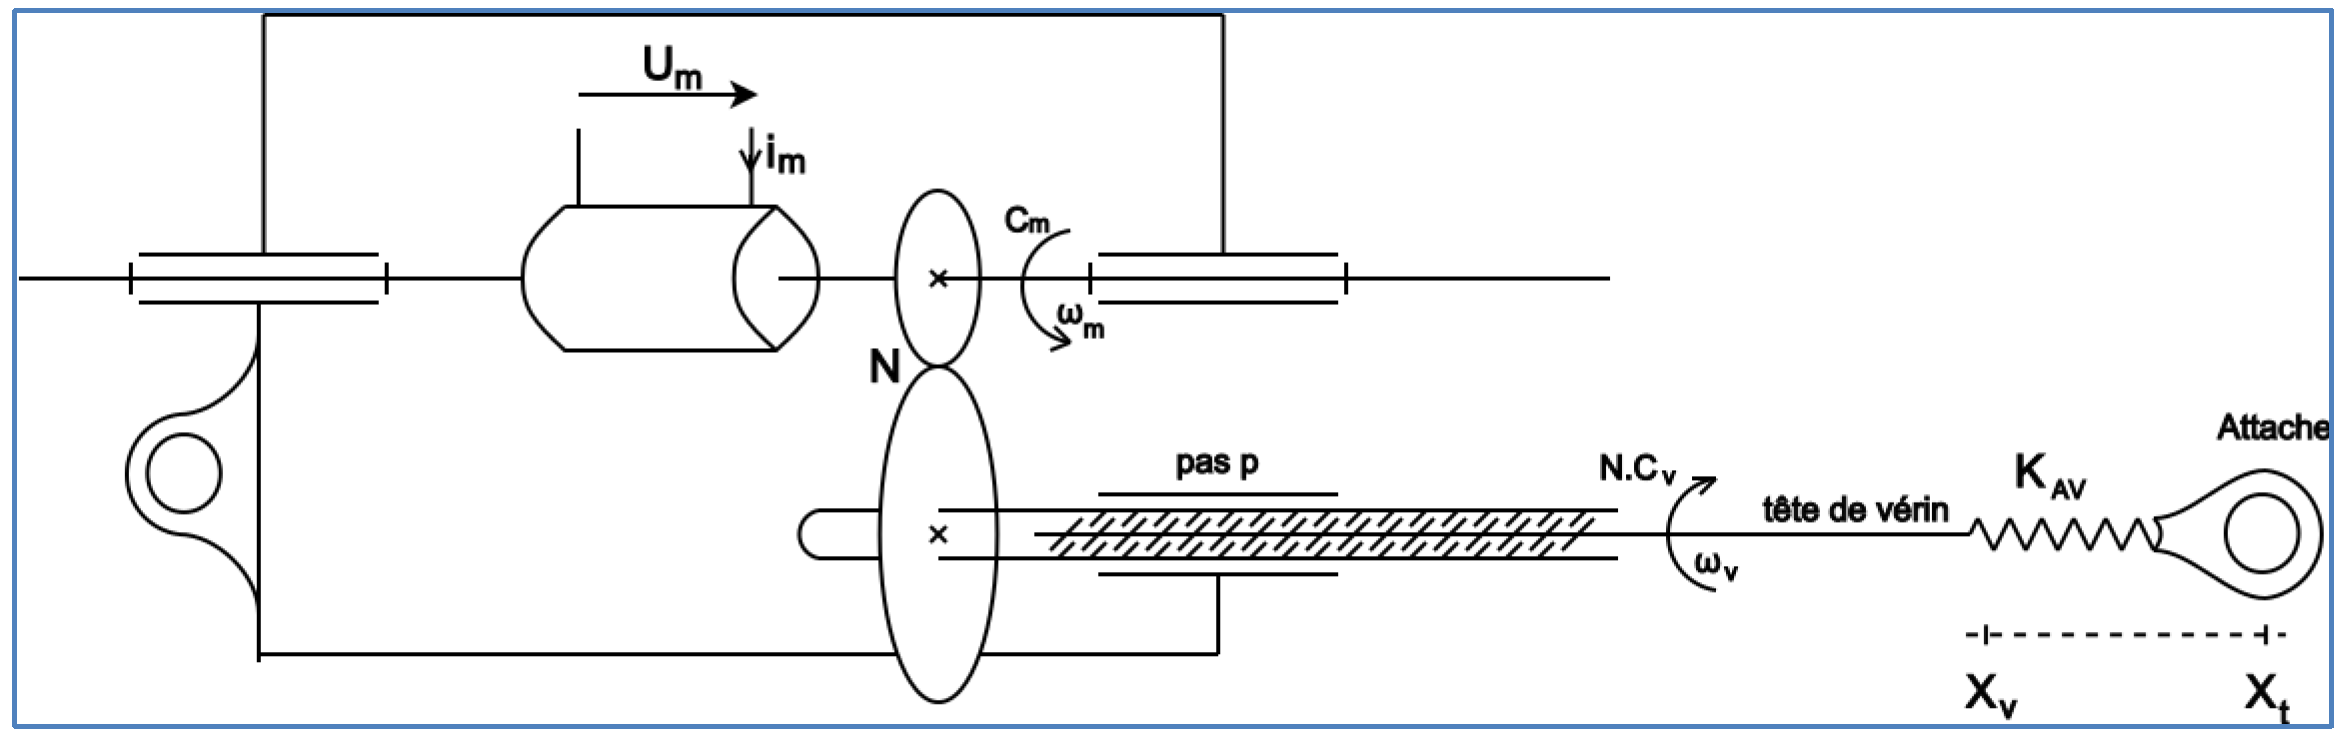
\includegraphics[width=0.7\linewidth]{img/fig15}
 \caption{Moteur}
 \label{img15}
\end{figure}

Le schéma de Laplace modélisant le moteur est proposé ci-dessous :

\begin{figure}[!h]
 \centering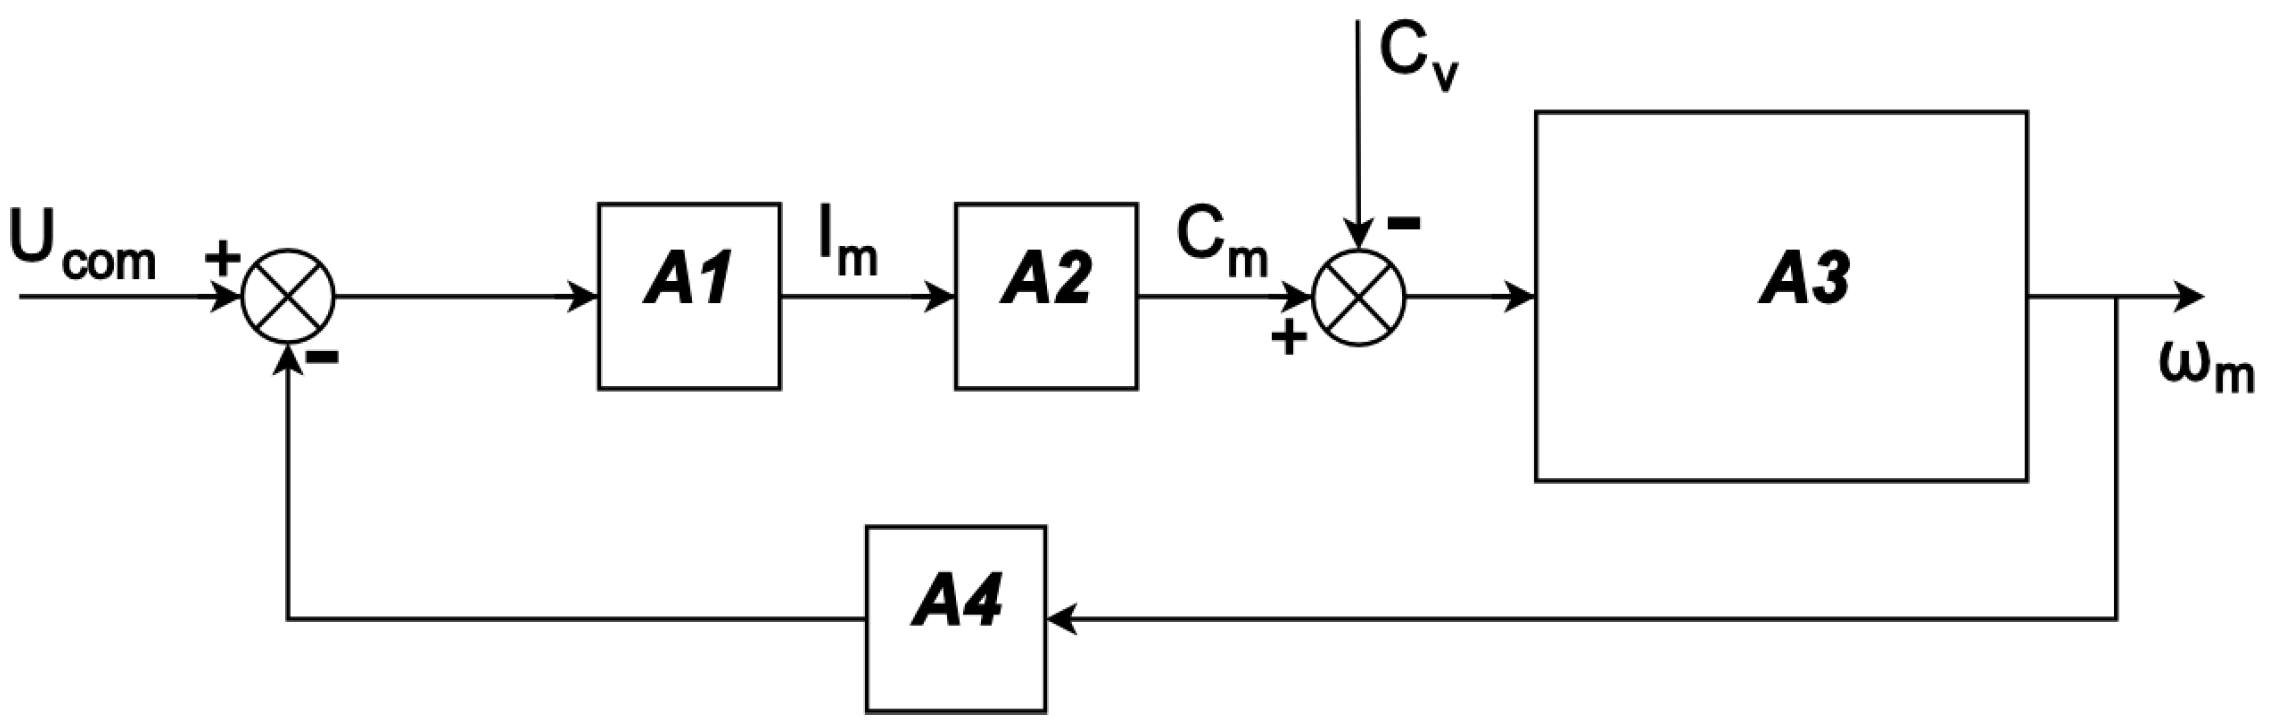
\includegraphics[width=0.7\linewidth]{img/fig18}
 \caption{Schéma de Laplace du moteur}
 \label{img18}
\end{figure}

\begin{table}[ht!]
\begin{tabular}{|l|l|}
\hline
$K=1,9Vs/rd (ou Nm/A)$ &constante de couple et de fem du moteur MCC \\
\hline
$N=3,04$ & rapport de réduction: $\omega_m/\omega_V$ \\
\hline
$f_v=0,182Nms/rd$ & coefficient de frottements fluides du pas de vis \\
\hline
$f_m=0,01Nms/rd$ & coefficient de frottements fluides du moteur \\
\hline
$p=10mm$ & pas du moteur en mm\\
\hline
$\lambda$ & pas du moteur en m/rd \\
\hline
\end{tabular}
 \caption{Données du système}
 \label{donnees_moteur}
\end{table}

On notera $\tau_v=\frac{J_{eq}}{f_m}$. On donne: $C_m(t)=f_m.\omega_m(t)+J_{eq}.\frac{d\omega_m(t)}{dt}+C_v(t)$.

\question{Expliciter $A_1(p)$, $A_2(p)$, $A_3(p)$ et $A_4(p)$ en fonction de la variable de Laplace p et des paramètres du moteur. On négligera l'inductance d'induit $L_m$.}

~\

D'après la Figure \ref{img15}, il est possible de calculer l'effort appliqué sur l'actionneur en fonction de la déformation de la liaison entre la tête de l'actionneur et l'attache de la traverse.

\begin{itemize}
 \item $K_{AV} = 5.10^7 N.m^{-1}$: raideur d'attache de la tête de l'actionneur,
 \item $X_V$: position de la vis (tête de l'actionneur),
 \item $X_T$: position de la traverse au niveau de l'attache. 
\end{itemize}

On donne $F_V=K_{AV}.(X_V-X_T)$.

\question{Déterminer les fonctions $A_5$ et $A_6$, avec $A_6=A_5$ en fonction des paramètres de la vis et du réducteur.}

\begin{figure}[!h]
 \centering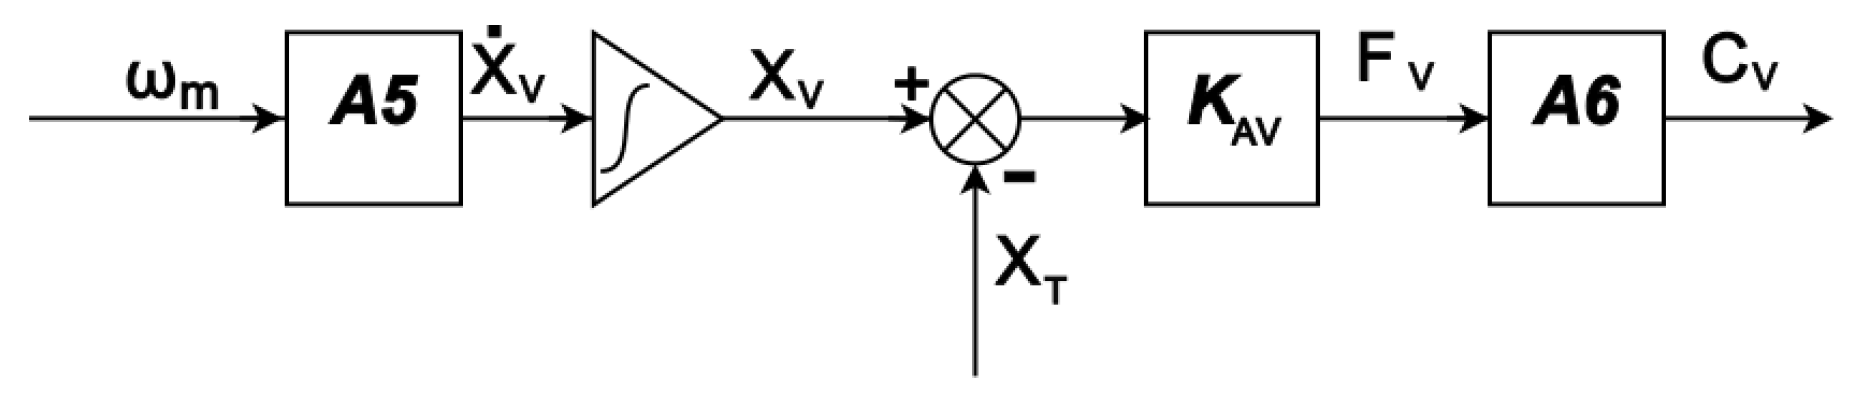
\includegraphics[width=0.5\linewidth]{img/fig19}
 \caption{Schéma de Laplace du réducteur et de l'actionneur}
 \label{img19}
\end{figure}

\paragraph{On cherche la fonction de transfert de l'actionneur.}

~\

Pour cela, on décompose le système (le schéma complet est donné figure \ref{img20}) en deux fonctions distinctes.

\question{Déduire des questions précédentes les fonctions de transfert suivantes : $\frac{F_V}{I_m}(p)_{X_T(p)=0}$ et $\frac{F_V}{X_T}(p)_{I_m(p)=0}$.}

\begin{figure}[!h]
 \centering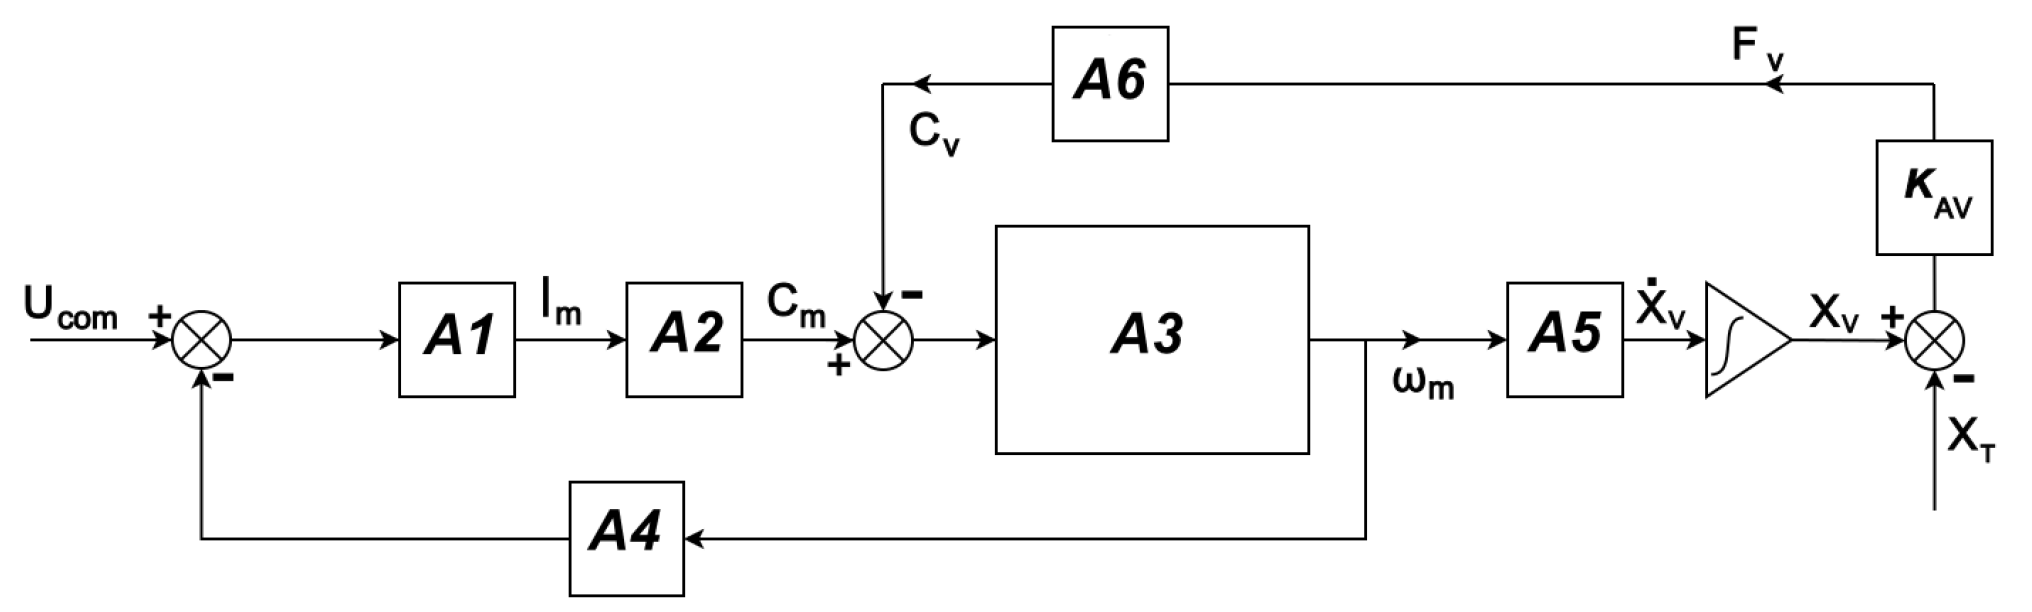
\includegraphics[width=0.8\linewidth]{img/fig20}
 \caption{Schéma de Laplace de l'actionneur détaillé}
 \label{img20}
\end{figure}

\question{Compléter le schéma bloc de l'actionneur complet en identifiant $A_7$, $A_8$ et $A_9$}.

\begin{figure}[!h]
 \centering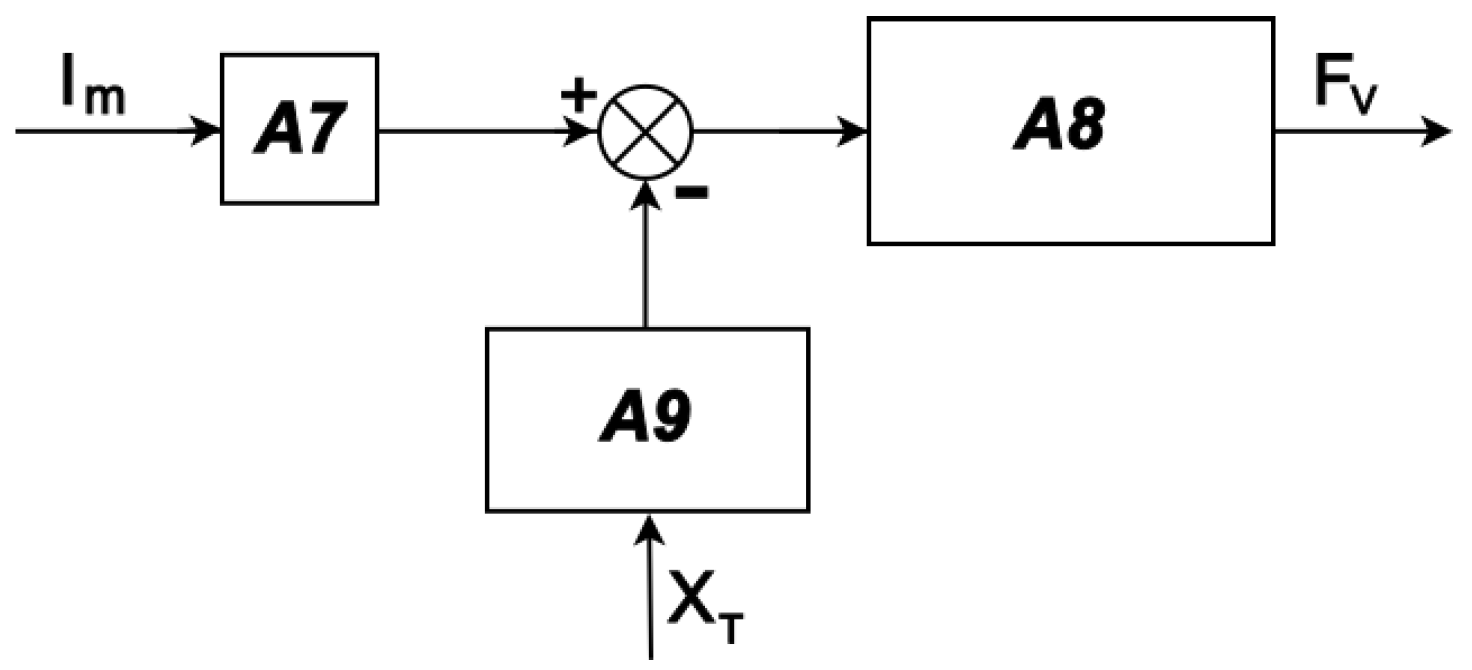
\includegraphics[width=0.4\linewidth]{img/fig21}
 \caption{Schéma de Laplace de l'actionneur complet}
 \label{img21}
\end{figure}

\question{Déterminer, à partir de la réponse Q18, l'expression de $F_V$ en statique (p $\rightarrow$ 0) en fonction de $I_m$.}

On peut montrer que: $C_m=F_v.\frac{\lambda}{N}+\left(\frac{f_v}{N^2}+f_m\right).\omega_m$.

\question{Montrer que le résultat à la question précédente peut être retrouvé avec cette indication.}

On s'intéresse à présent à la commande en tension ($U_{com}$) du moteur.

\question{On cherche la fonction de transfert liant $X_V$ à $U_{com}$.}

\begin{enumerate}
 \item Exprimer $\omega_m(p)$ en fonction de $I_m$ et $F_V$. (revoir Q16 et Q17),
 \item Exprimer $X_V(p)$ en fonction de $\omega_m$. (revoir Q17).

\begin{figure}[!h]
 \centering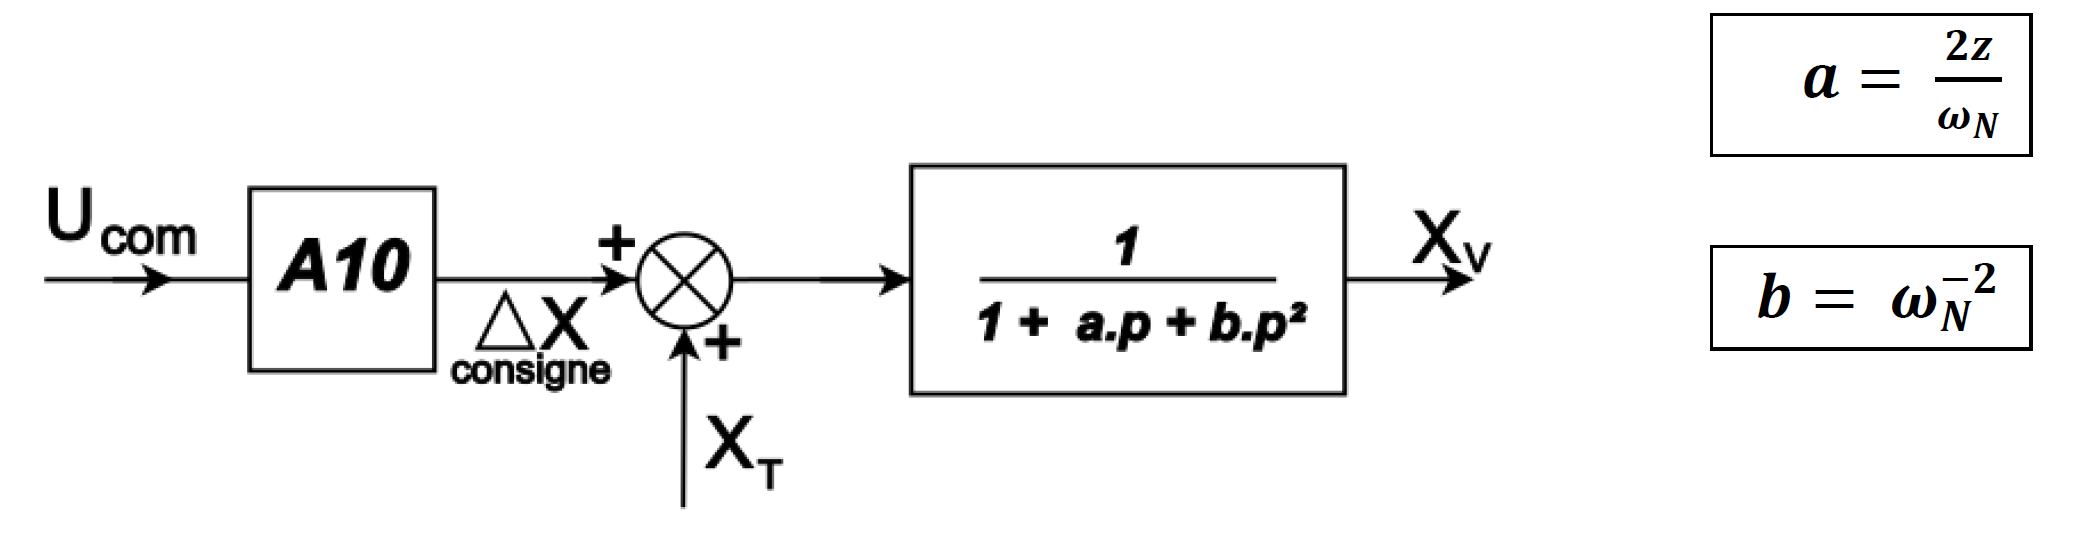
\includegraphics[width=0.7\linewidth]{img/fig22}
 \caption{Schéma de Laplace de l'actionneur complet du point de vue de la commande}
 \label{img22}
\end{figure}
 \item En déduire, à partir des résultats 1 et 2, la relation entre $X_V$ et $U_{com}$.
\end{enumerate}

\question{Identifier $A_{10}$, $\omega_N$ et $z$ à partir des résultats précédents.}

\question{Donner la condition permettant d'éviter un dépassement afin de répondre au cahier des charges.}

\section{Vérification de la précision de positionnement}

On se propose dans cette partie de vérifier la précision de pendulation.

Le cahier des charges spécifie que sur une consigne de position, la course de l'axe de l'actionneur ne doit présenter aucune \og marche \fg supérieure à 2 mm.

La course effectuée par l'axe de l'actionneur est connue grâce à un boitier de recopie de type capteur résolveur monté à l'extrémité de l'axe moteur.

La réduction utilisée est de $100(\frac{\omega_m}{\omega_{res}}=100$) entre la rotation de l'axe moteur et celle du capteur résolveur. Le pas de la vis est $p=10mm$.

\question{Déterminer la rotation qu'effectue le capteur résolveur pour la course maximale de l'axe actionneur de 140 mm.}

\question{Justifier alors le choix de ce rapport de réduction.}

L'incertitude sur le calage du zéro résolveur est de $\pm10$ minute d'angle.

Définition des différents jeux dans la chaîne d'actionneur :
\begin{itemize}
 \item articulations actionneur/bogie et actionneur/traverse : $\Delta_{art}=\pm0,12mm$,
 \item jeu au niveau du couple d'engrenages du réducteur : $\Delta_{red}=\pm0,2\degree$,
 \item jeu pour la vis à rouleau : $\Delta_{vis}=\pm0,02mm$.
\end{itemize}

\question{Exprimer la course de l'actionneur $X_v$ en fonction de l'angle $\alpha_{rec}$ du capteur résolveur en intégrant les différents jeux.}

\question{En déduire la précision de positionnement de l'axe de l'actionneur pour une course de 140 mm et conclure vis-à-vis du cahier des charges.}

\section{Conception de la liaison entre l'entrainement et l'axe roue du bogie}

La figure \ref{img23} présente une vue 3D d'un axe de roue du bogie, on y voit les deux roues et les deux pignons qui permettent d'entrainer l'arbre.

\begin{figure}[!h]
 \centering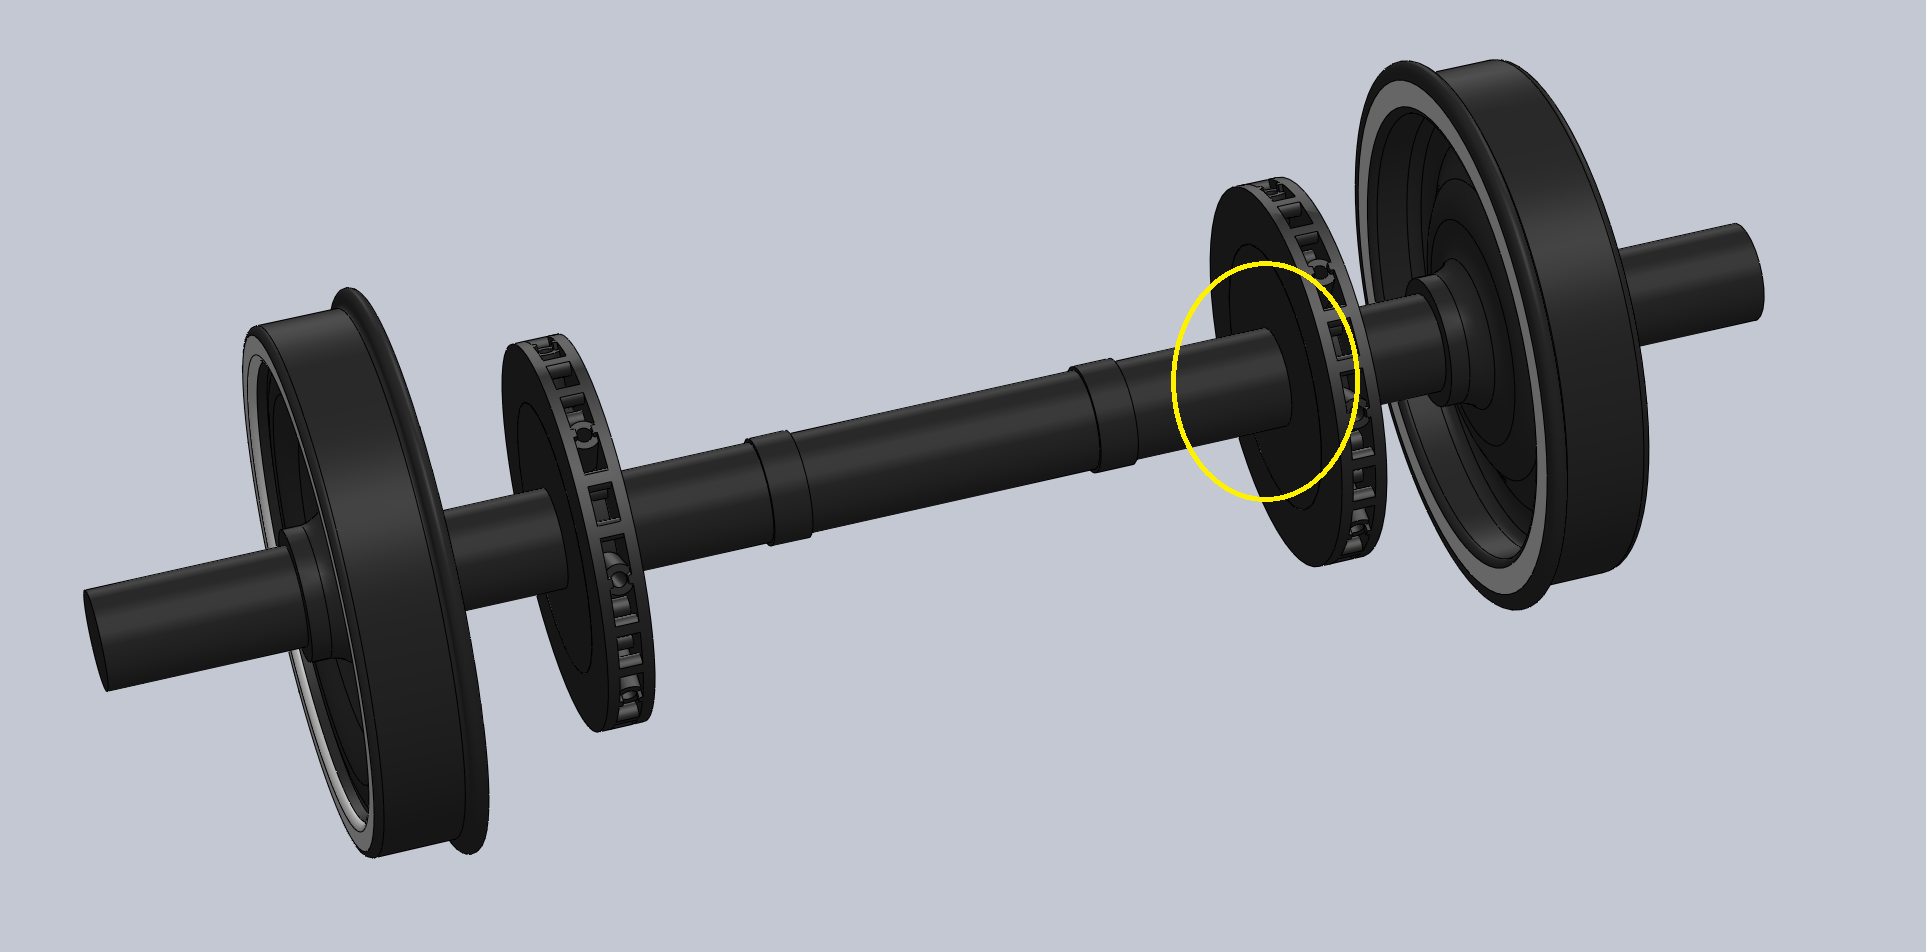
\includegraphics[width=0.6\linewidth]{img/fig23}
 \caption{Vue 3D d'un train du bogie}
 \label{img23}
\end{figure}

On s'intéresse à la liaison entre l'engrenage et l'axe, entourée sur la figure \ref{img23}.

\begin{figure}[!h]
 \centering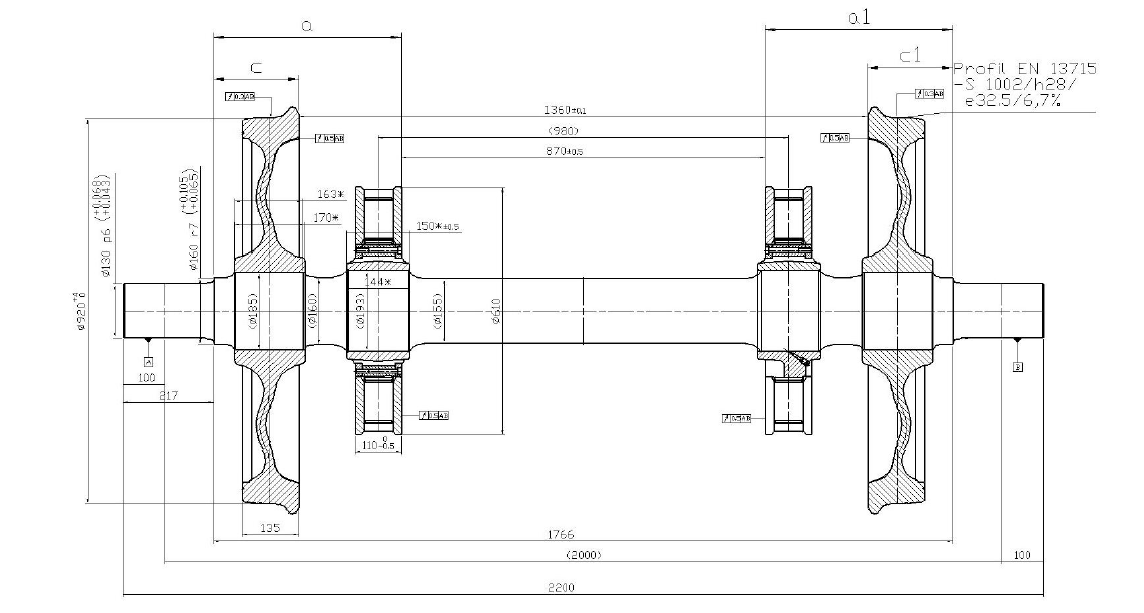
\includegraphics[width=0.9\linewidth]{img/fig24}
 \caption{Plan d'un train du bogie}
 \label{img24}
\end{figure}

La figure \ref{img24} montre la solution actuelle d'assemblage. L'engrenage est monté en force et la liaison n'est pas démontable. Or, il arrive que l'engrenage casse et à ce moment là, tout le train doit être remplacé. On souhaite donc une solution démontable comme celle entre l'arbre et le roulement présentée à la figure \ref{img25}. On ajoutera une clavette afin de bloquer la rotation de l'engrenage autour de l'arbre.

\begin{figure}[!h]
 \centering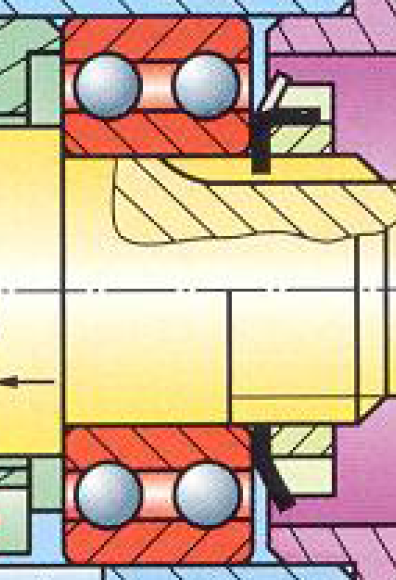
\includegraphics[width=0.4\linewidth]{img/fig25}
 \caption{Solution d'assemblage}
 \label{img25}
\end{figure}

\question{Compléter le dessin du document réponse en intégrant cette solution pour l'assemblage de l'engrenage.}

~\

Détail de la conception:
\begin{itemize}
 \item intégrer une clavette,
 \item mettre un épaulement sur un des côté (faire attention à l'assemblage),
 \item mettre un écrou de l'autre côté (faire attention à l'assemblage).
\end{itemize}

\begin{center}
----- FIN DU SUJET -----
\end{center}

\cleardoublepage

\pagestyle{documentreponse}

\section{Documents réponse}

\reponse{13}

\reponse{0}

\vspace{-3cm}

\begin{center}
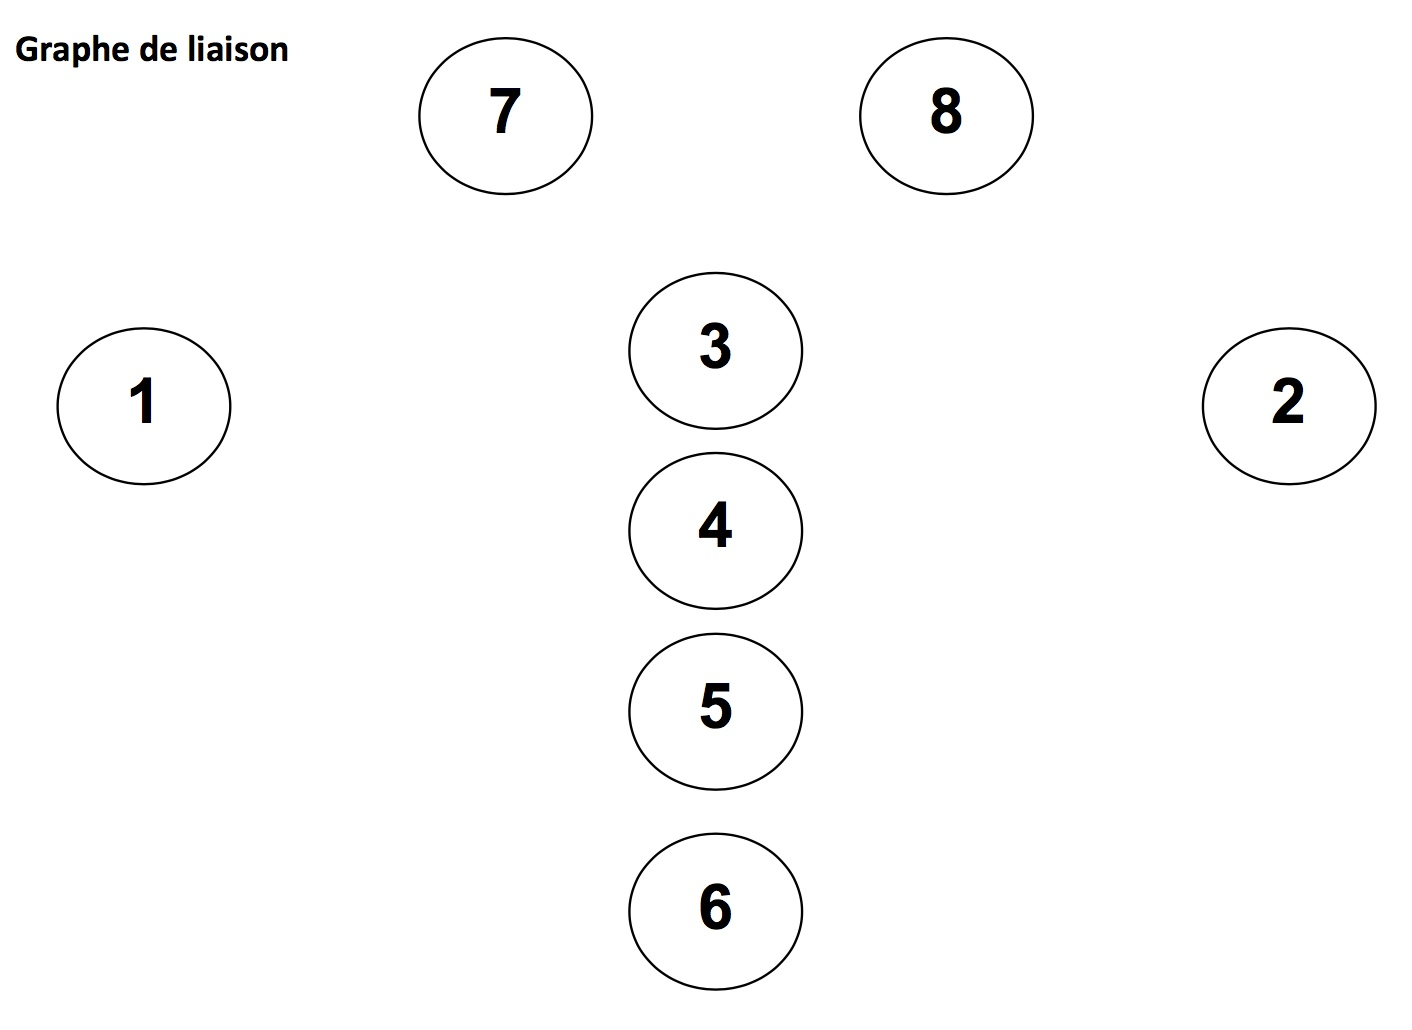
\includegraphics[width=0.6\linewidth]{img/Q1}
\end{center}

~\

\vspace{10cm}

\reponse{0}

\begin{center}
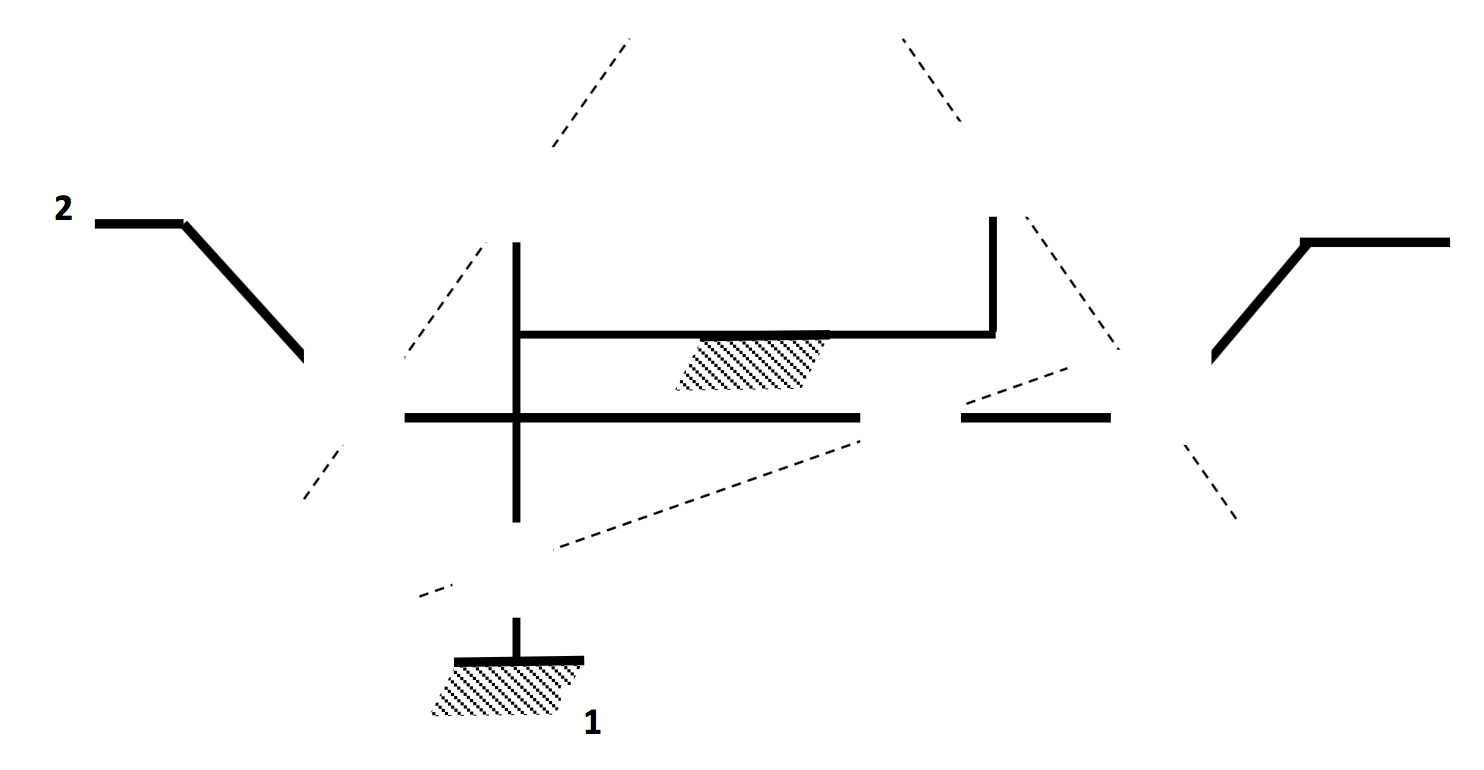
\includegraphics[width=0.6\linewidth]{img/Q2}
\end{center}

\reponse{13}

\reponse{13}

\newpage

\reponse{13}

\reponse{13}

\reponse{13}

\newpage

\reponse{0}

\begin{center}
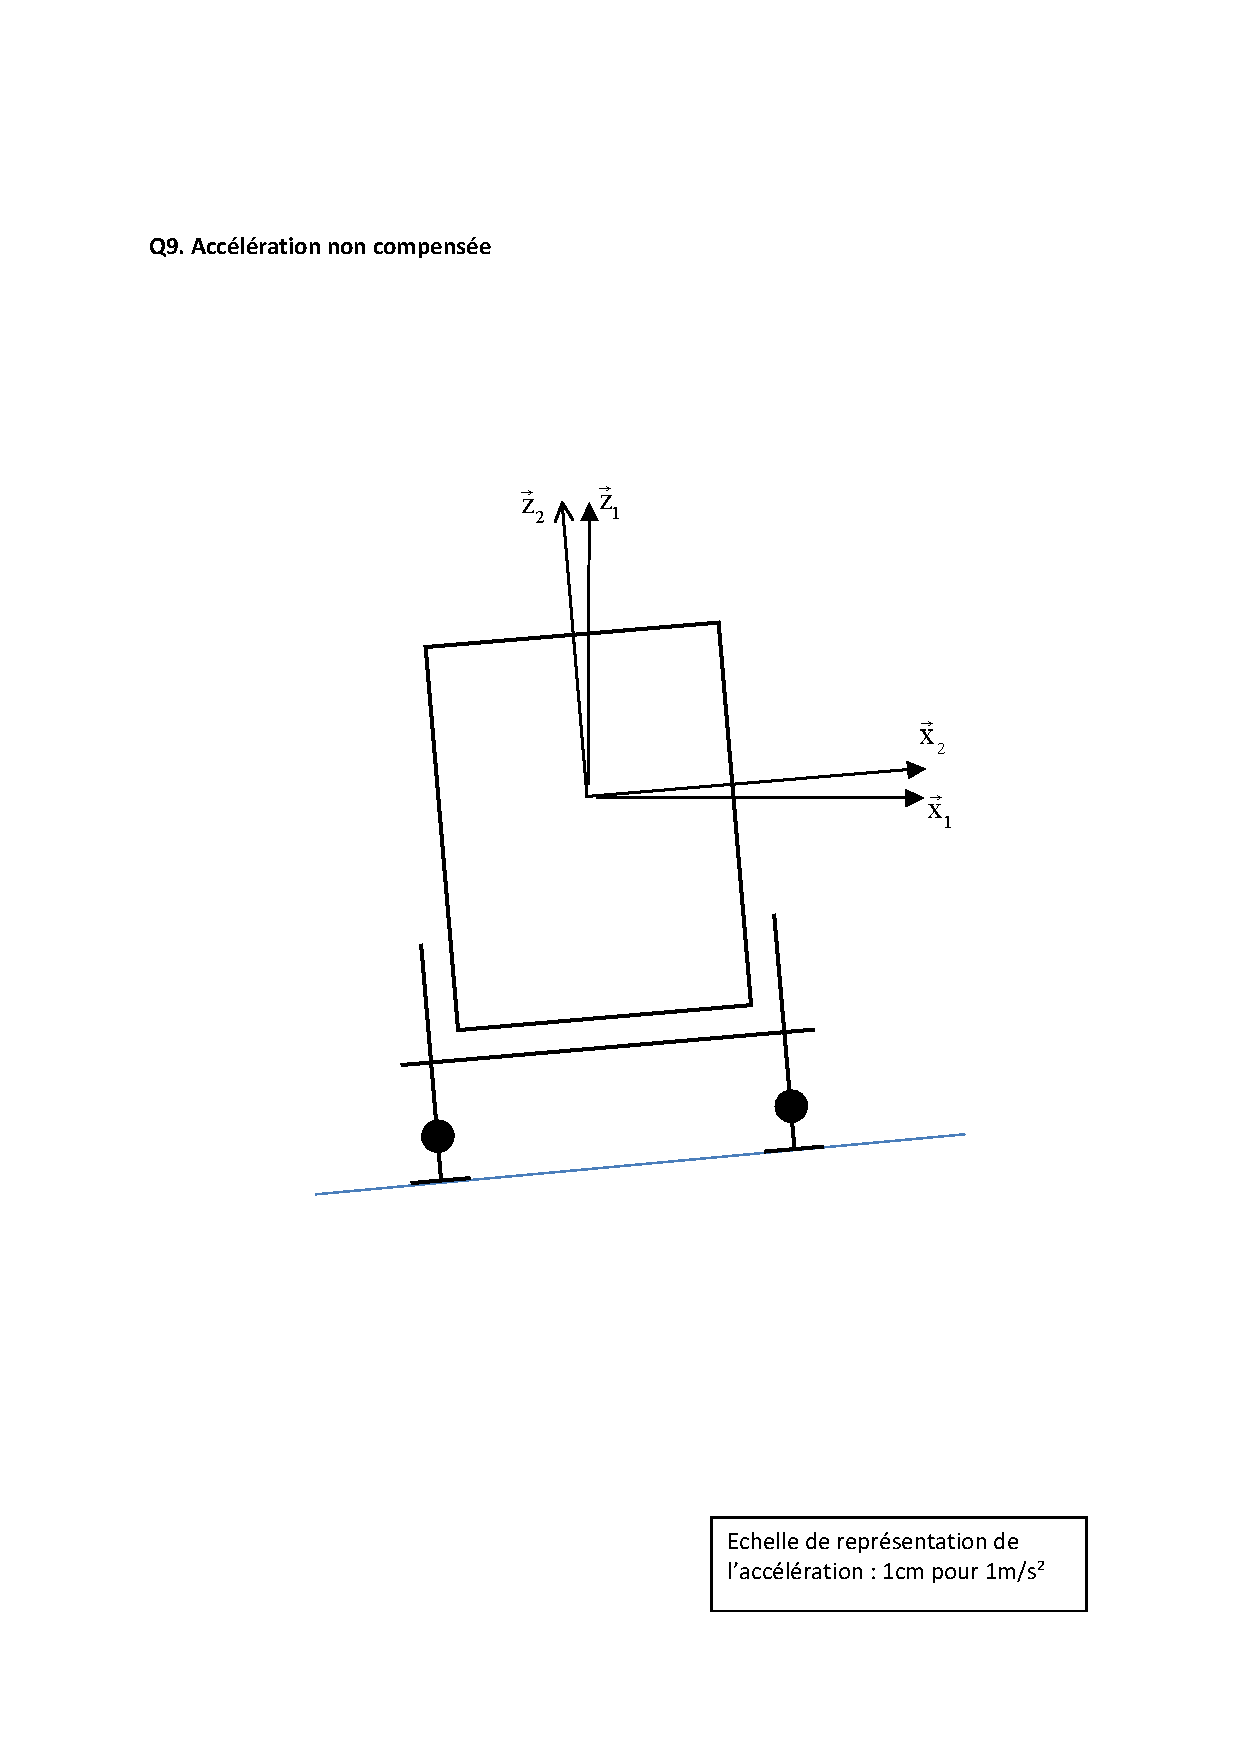
\includegraphics[width=0.9\linewidth]{img/Q3}
\end{center}

\newpage

\reponse{10}

\reponse{10}

\reponse{10}

\newpage

\reponse{0}

\begin{center}
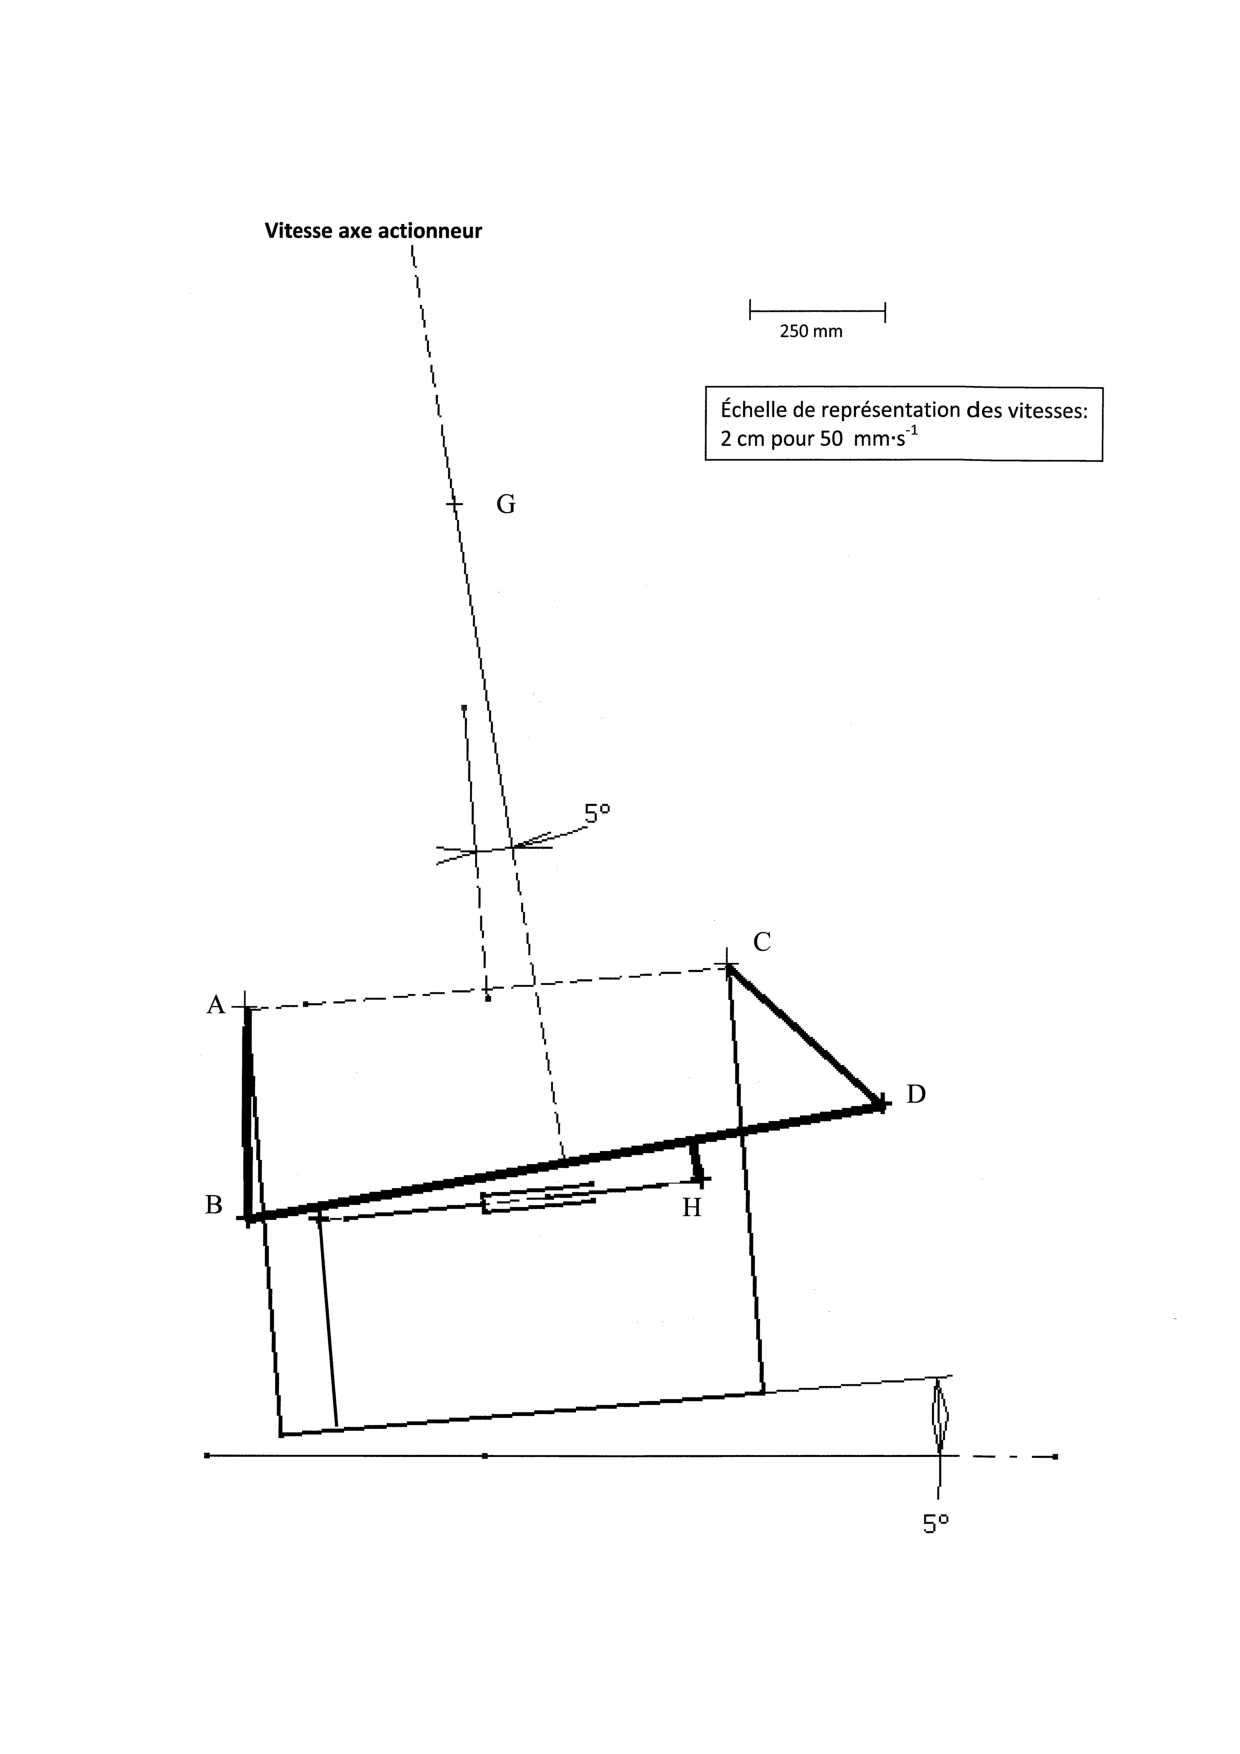
\includegraphics[width=0.9\linewidth]{img/Q4}
\end{center}

\newpage

\reponse{30}

\reponse{10}

\newpage

\reponse{10}

\reponse{10}

\reponse{20}

\newpage

\reponse{10}

\reponse{10}

\reponse{10}

\reponse{35}

\reponse{13}

\reponse{5}

\newpage

\reponse{7}

\reponse{7}

\reponse{7}

\reponse{10}

\newpage

\reponse{0}

\begin{center}
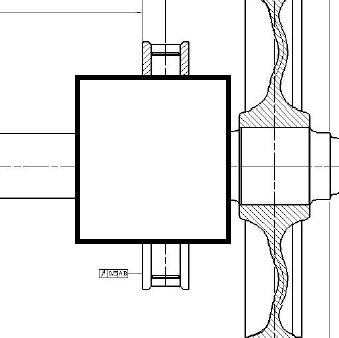
\includegraphics[width=0.9\linewidth]{img/Q5}
\end{center}

\ifdef{\public}{\end{document}}{}

\newpage
\cleardoublepage

\pagestyle{correction}

\setcounter{equation}{0}

\section{Correction}

\cor{\begin{itemize}
\item S.C.1: Traverse + 4 bielles montées en liaison pivot,
\item S.C.2: Moteur,
\item S.C.3: Réducteur,
\item S.C.4: Vis réversible.
\end{itemize}}

\cor{\begin{center}
 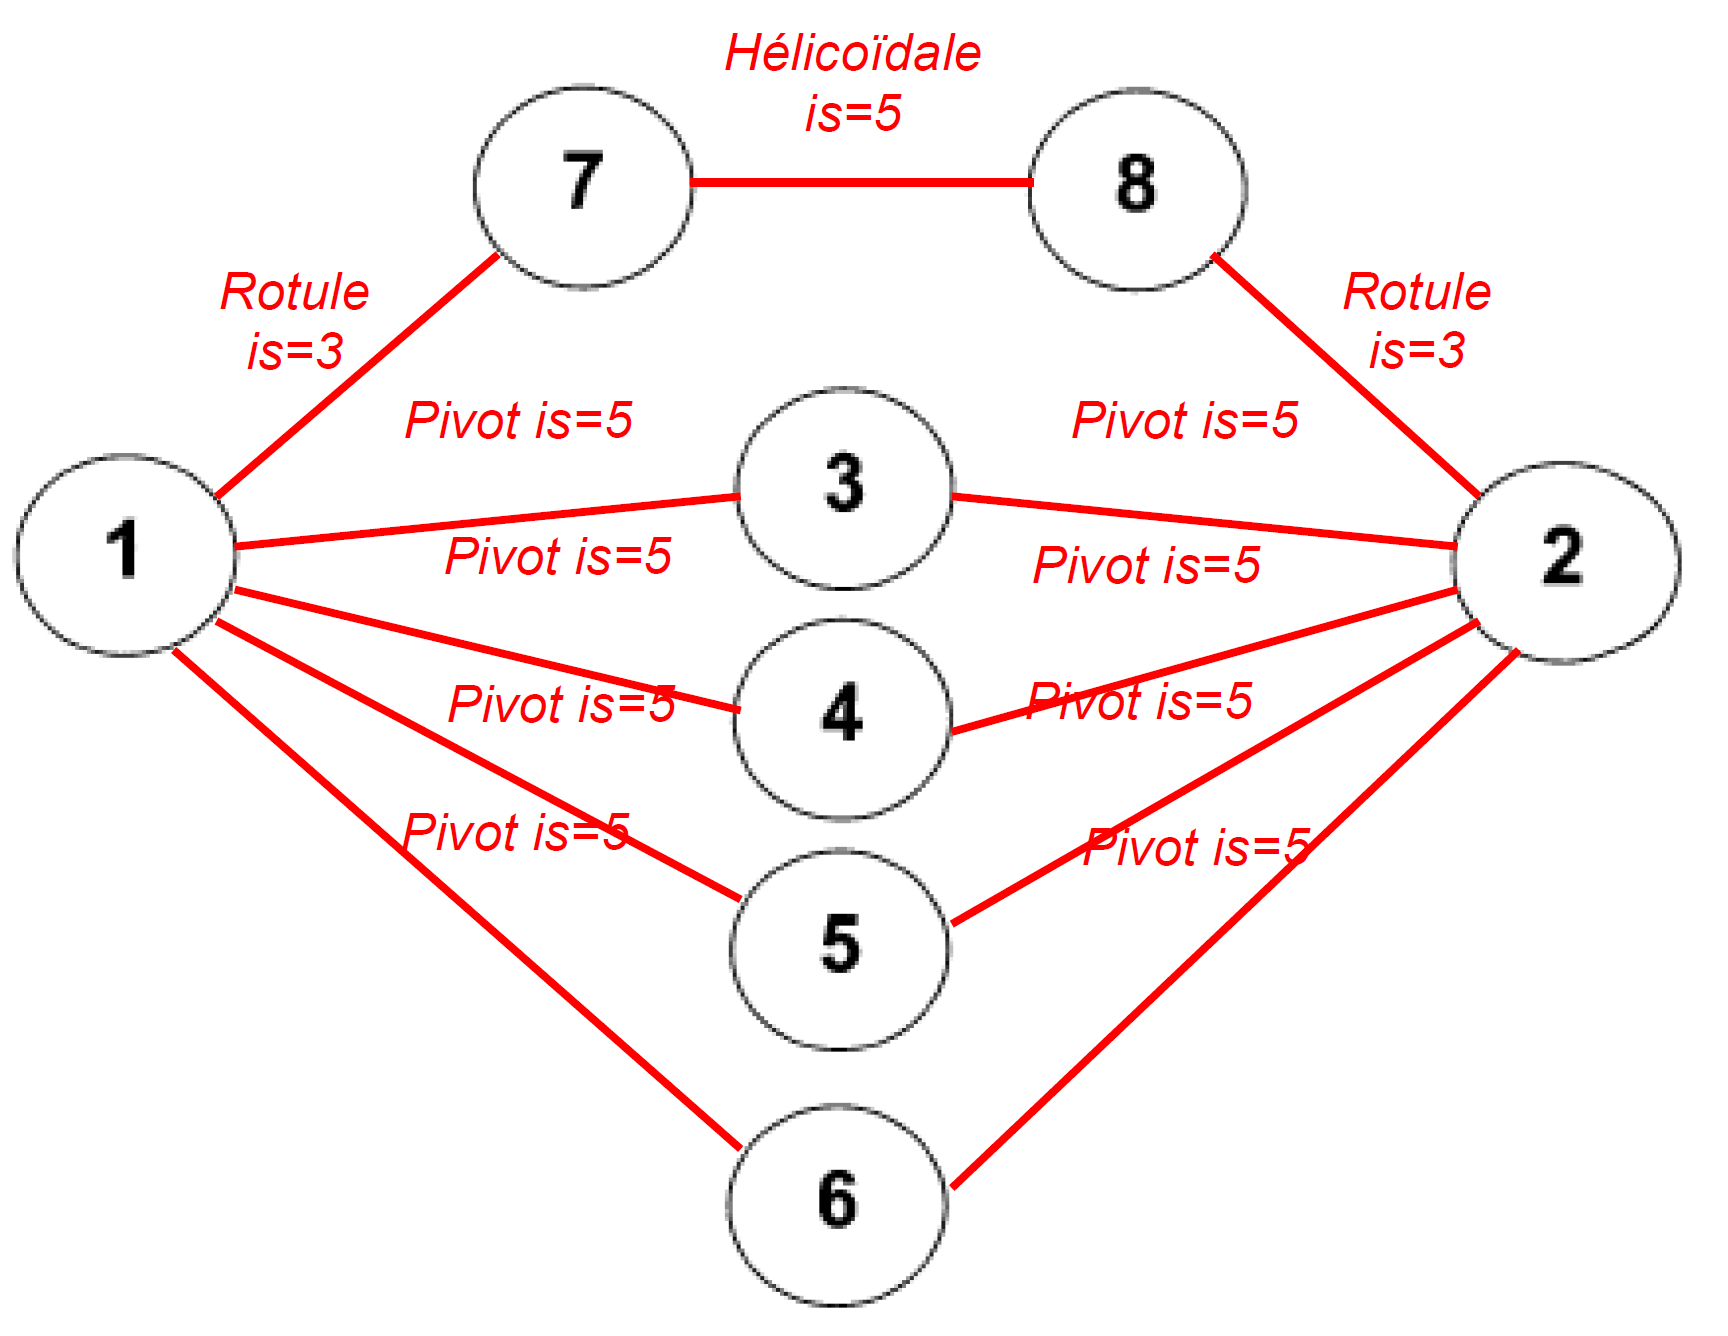
\includegraphics[width=0.8\linewidth]{img/COR1}
\end{center}}

\begin{itemize}
 \item Nombre de mobilités: mc = 2
 \item Nombre d'équations statiques: rs=6.(p-1)-mc=6.(8-1)-2= 42
 \item Nombre d'inconnues statiques: Ns = 8.5 + 5 + 2.3 = 51 (8 pivots, 1 hélicoïdale, 2 rotules)
 \item h=Ns-rs=11, donc le système est hyperstatique d'ordre 11
\end{itemize}

\cor{\begin{center}
 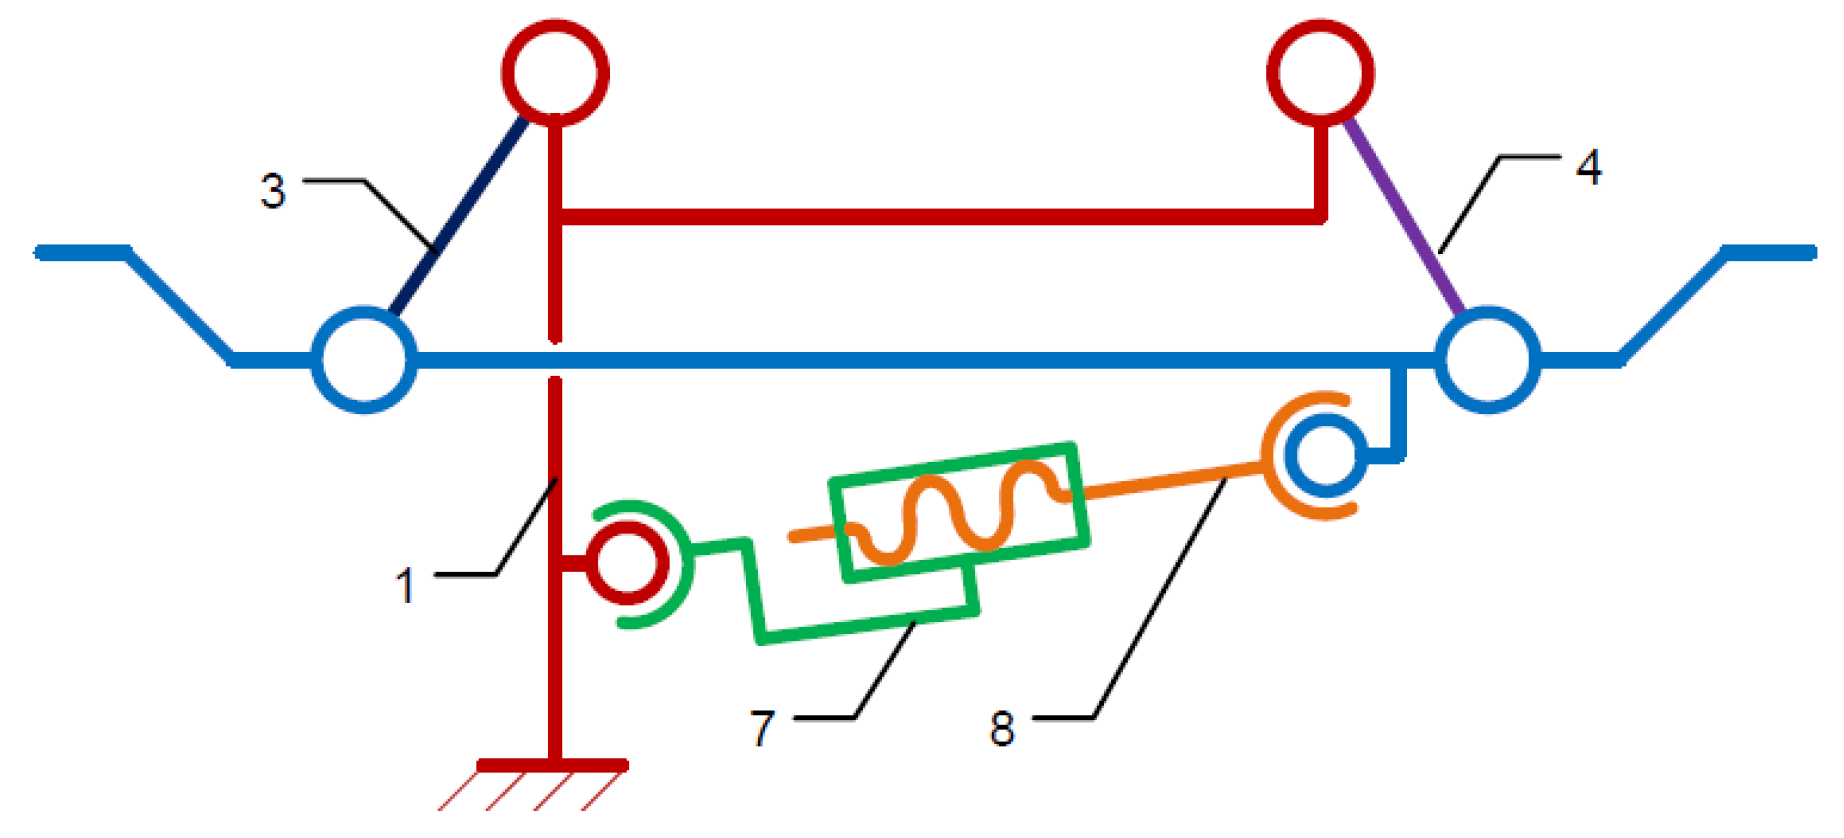
\includegraphics[width=0.8\linewidth]{img/COR2}
\end{center}}

\begin{itemize}
 \item Nombre de mobilités: mc = 2
 \item Nombre d'équations statiques: rs=6.(p-1)-mc=6.(6-1)-2= 28
 \item Nombre d'inconnues statiques: Ns = 4.5 + 5 + 2.3 = 31 (4 pivots, 1 hélicoïdale, 2 rotules)
 \item h=Ns-rs=3, donc le système est hyperstatique d'ordre 3
\end{itemize}

\cor{\begin{itemize}
 \item La liaison 3/2 doit être // à la liaison 6/2,
 \item La liaison 4/2 doit être // à la liaison 6/2,
 \item La liaison 5/2 doit être // à la liaison 6/2,
 \item La liaison 3/2 doit être coaxiale à la liaison 6/2,
 \item La liaison 4/2 doit être coaxiale à la liaison 5/2.
\end{itemize}}

\cor{$\overrightarrow{a_{G/R0}}=\left[\frac{d\overrightarrow{v_{G/R0}}}{dt}\right]_{R0}=\left[\frac{dV.\overrightarrow{y_1}}{dt}\right]_{R0}=\overrightarrow{\Omega_{R1/R0}}\wedge V.\overrightarrow{y_1}=-\dot{\theta}.V.\overrightarrow{x_1}$}

Avec $\dot{\theta}=\frac{V}{R}$, on obtient $\overrightarrow{a_{G/R0}}=-\frac{V^2}{R}.\overrightarrow{x_1}$

\cor{$\gamma_{nc}=(\vec{g}-\overrightarrow{a_{G/R0}}).\overrightarrow{x_2}=(-g.\overrightarrow{z_0}+\frac{V^2}{R}.\overrightarrow{x_1}).\overrightarrow{x_2}=-g.sin\delta+\frac{V^2}{R}.cos\delta$

On a: $cos\delta=1$ et $sin\delta=\frac{d}{e}$, donc:

$\gamma_{nc}=\frac{V^2}{R}-g.\frac{d}{e}$}

\cor{On veut $\gamma_{nc}=0$, donc $d=\frac{V^2.e}{R.g}$, donc $\delta=arcsin\left(\frac{V^2}{R.g}\right)$}

\cor{Application numérique: $\gamma_{nc}=\frac{\left(\frac{145.1000}{60.60}\right)^2}{800}-\frac{10.100}{1150}=1,16m.s^{-2}$}

\newpage

\cor{\begin{center}
 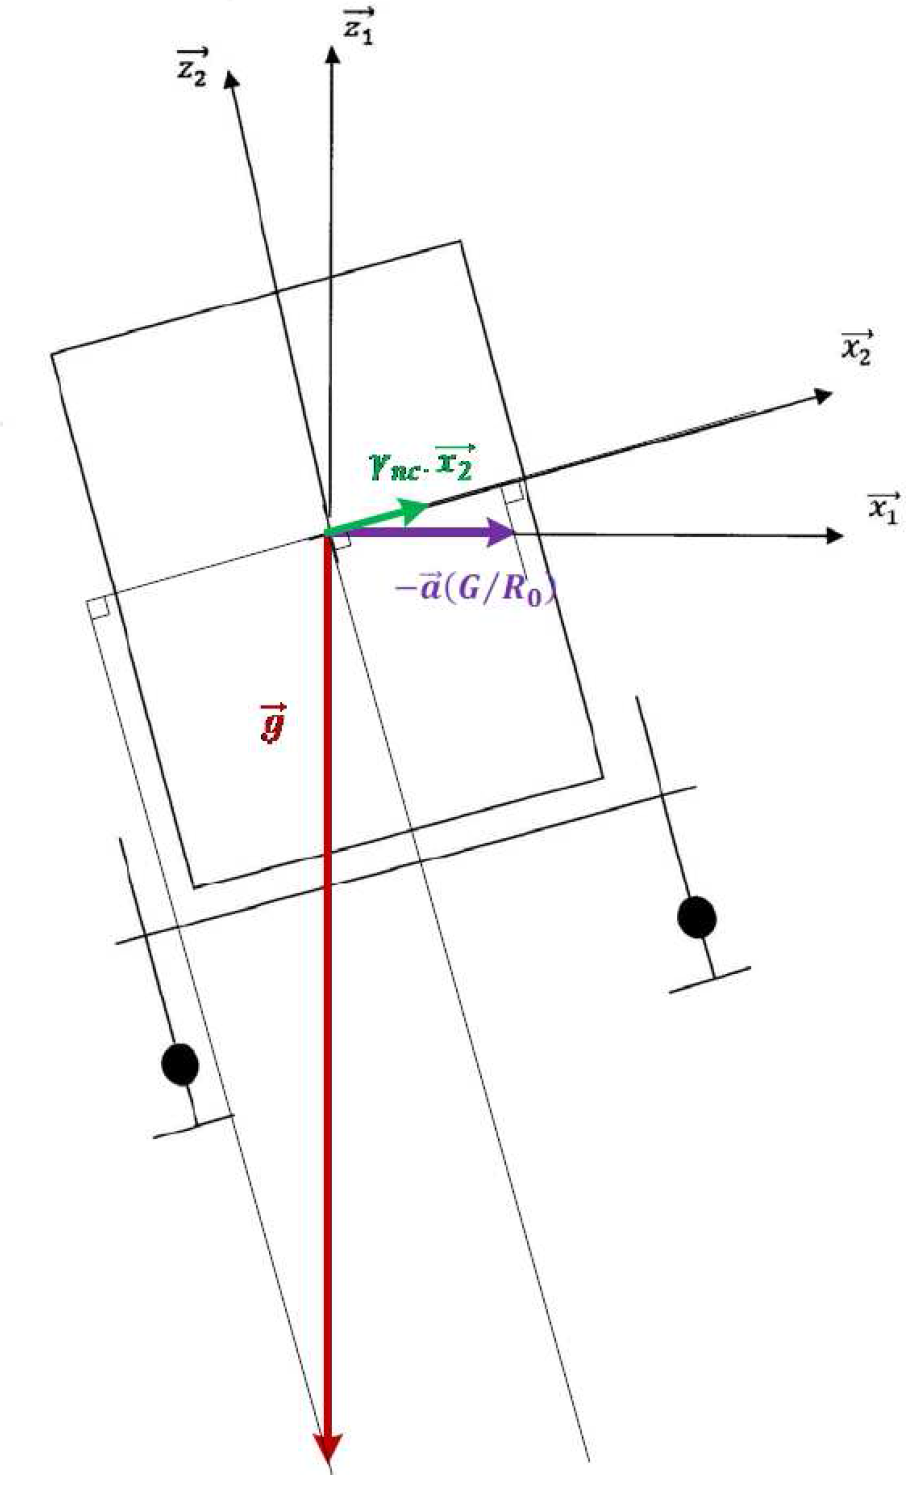
\includegraphics[width=0.5\linewidth]{img/COR3}
\end{center}}

\cor{D'après la question 7, $d=\frac{V^2.e}{R.g}=\frac{40,3^2+1150}{800.10}=233,5mm$

Sachant que le dévers actuel fait 100mm, l'insuffisance de dévers vaut donc $233,5-100=133,5mm$.

$\delta=arcsin\left(\frac{d}{e}\right)=11,7\degree$}

\cor{D'après la question 6, $\gamma_{nc}=\frac{V^2}{R}-g.sin(\delta+\alpha)$

On a donc $\frac{V^2}{R}=\gamma_{nc}+g.sin(\delta+\alpha)$, donc $V=\sqrt{R.(\gamma_{nc}+g.sin(\delta+\alpha))}$

$V=\sqrt{800.(1,2+10.0,31)}=\sqrt{800.4,3}\simeq40.\sqrt{2}\simeq56m.s^{-1}\simeq200km.h^{-1}$}

\cor{$sin\delta\simeq0,2$, donc $V=\sqrt{800.(1,2+10.0,2)}=\sqrt{80.32}\simeq16.\sqrt{10}\simeq48m.s^{-1}\simeq172km.h^{-1}$

Pour parcourir 100km, à $172km.h^-1$, il faut 0,58h.

Pour parcourir 100km, à $200km.h^-1$, il faut 0,5h.

Le gain est donc de $\frac{0,58-0,5}{0,5}.100=16\%$, le cahier des charges est donc respecté.}

\cor{\begin{center}
 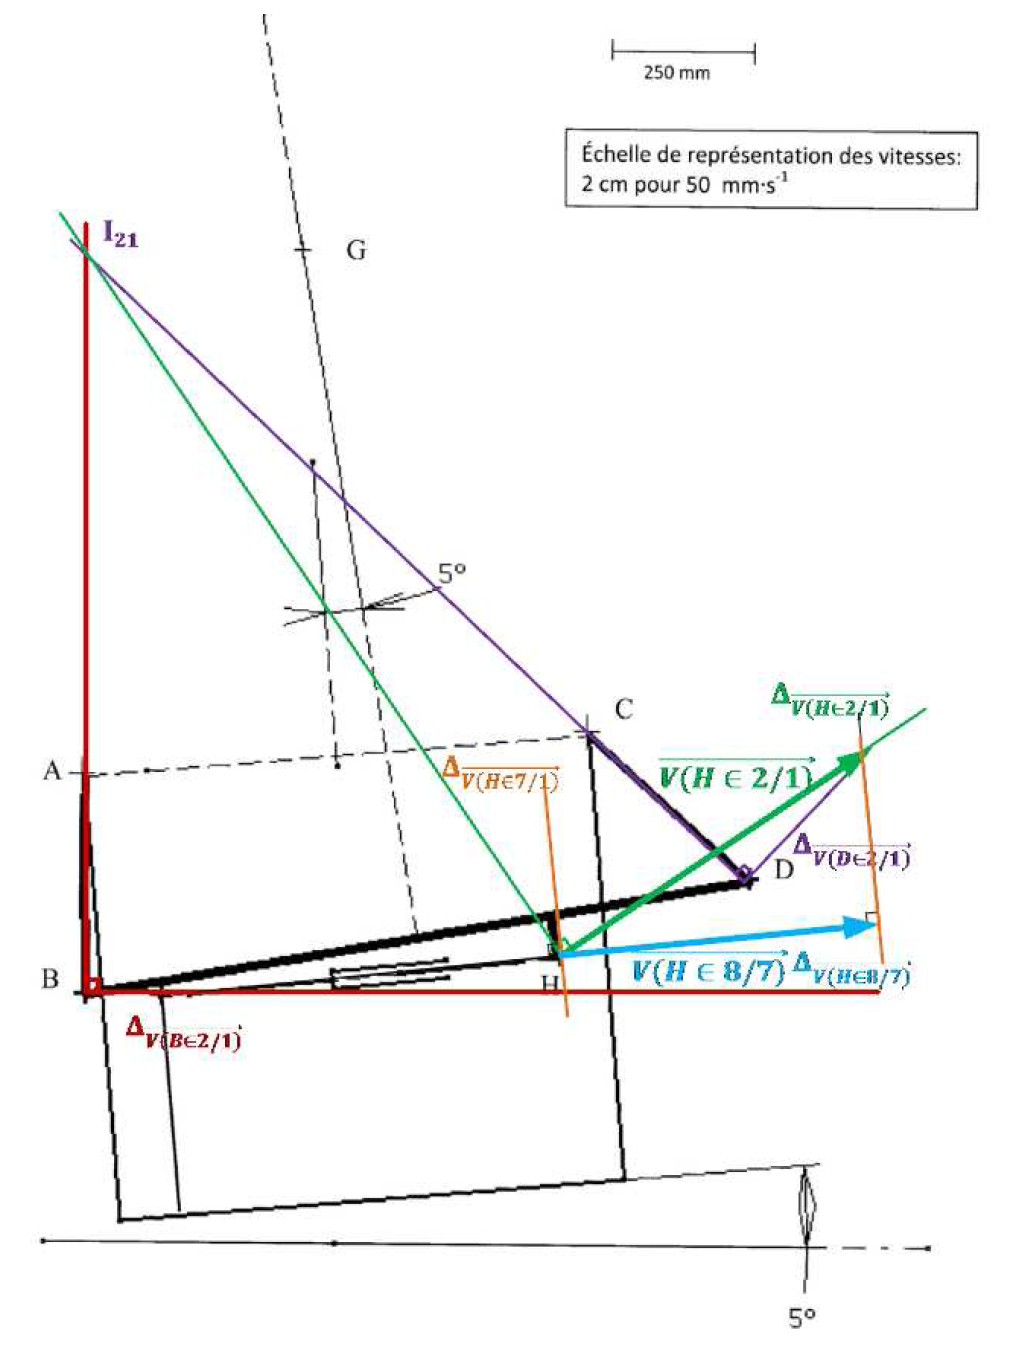
\includegraphics[width=0.5\linewidth]{img/COR4}
\end{center}}

\cor{$t\in[0;0,12]$, $V(t)=1000.t$, donc $X_v(t)=1000.\frac{t^2}{2}$, avec $X_v(0,12)=1000.\frac{0,12^2}{2}=7,2$

~\

$t\in[0,12;1,08]$, $V(t)=120$, donc $X_v(t)=120.t+C_0$, avec $X_v(0,12)=120.0,12+C_0=7,2$, donc $C_0=-7,2$, donc $X_v(t)=120.t-7,2$ et $X_v(1,08)=120.1,08-7,2=122,4$.

~\

$t\in[1,08;1,2]$, $V(t)=-1000.t+C_1$, avec $V(1,2)=-1000.1,2+C_1=0$, donc $C_1=1200$ donc $X_v(t)=-1000.\frac{t^2}{2}+1200.t+C_2$, avec $X_v(1,08)=-1000.\frac{1,08^2}{2}+1200.1,08+C_2=122,4$, donc $C_2=-590,4$, donc $X_v(t)=-1000.\frac{t^2}{2}+1200.t-590,4$}

\cor{$X_{total}=-1000.\frac{1,2^2}{2}+1200.1,2-590,4=-720+1440-590,4=129,6mm$

$X_{total}=120*1,08=129,6mm$}

\cor{$A_1(p)=\frac{1}{R}$, $A_2(p)=K$, $A_3(p)=\frac{1}{J_{eq}.p+f_r}$, $A_4(p)=K$}

\cor{$\frac{dX_v}{dt}=\frac{\lambda}{N}.\omega_m$, donc $p.X_v(p)=\frac{\lambda}{N}.\omega_m(p)$, donc $A_5(p)=A_6(p)=\frac{\lambda}{N}$}

\cor{$\frac{F_v}{I_m}(p)=\frac{K_{AV}.A5.A3.A2}{p+K_{AV}.A5.A3.A6}$ et $\frac{F_v}{X_T}(p)=-\frac{p.K_{AV}}{p+K_{AV}.A5.A3.A6}$}

\cor{$F_v=\frac{K_{AV}}{p+K_{AV}.A5.A3.A6}.(A5.A3.A2.I_m-p.X_T)=A8.(A7.I_m-A9.X_T)$,

donc $A7=A5.A3.A2$, $A8=\frac{K_{AV}}{p+K_{AV}.A5.A3.A6}$ et $A9=p$}

\cor{$\frac{F_V}{I_m}(p)=\frac{K_{AV}.\frac{\lambda}{N}.\frac{1}{f_m}.\frac{1}{\tau_v.p+1}.K}{p+K_{AV}.\frac{\lambda}{N}.\frac{1}{f_m}.\frac{1}{\tau_v.p+1}.\frac{\lambda}{N}}$

En statique, $p\rightarrow 0$, donc $\frac{F_V}{I_m}(p)\rightarrow \frac{K.N}{\lambda}$}

\cor{En statique $\omega_m=0$, donc $C_m=K.I_m\rightarrow F_v.\frac{\lambda}{N}$, donc $\frac{F_V}{I_m}(p)\rightarrow \frac{K.N}{\lambda}$}

\cor{$\omega_m=A3.(A2.I_m-A6.F_v)=A3.A2.I_m-A3.A6.F_v$

$X_v=\frac{A5}{p}.\omega_m$

$X_v=\frac{A5}{p}.A3.A2.I_m-\frac{A5}{p}.A3.A6.F_v=\frac{A5}{p}.A3.A2.A1.(U_{com}-A4.\omega_m)-\frac{A5}{p}.A3.A6.K_AV.(X_v-X_T)$

or $\omega_m=\frac{p}{A5}.X_V$,

donc $X_V=\frac{\frac{K.N}{R.\lambda.K_{AV}}.U_{com}+X_T}{1+\left(\frac{K^2.N^2}{R.\lambda^2.K_{AV}}+\frac{N^2.f_m}{\lambda^2.K_{AV}}\right).p+\frac{\tau_v.N^2.f_m}{\lambda^2.K_{AV}}.p^2}$}

\cor{$A10=\frac{K.N}{R.\lambda.K_{AV}}$, $\omega_N=\frac{\lambda}{N}.\sqrt{\frac{K_{AV}}{\tau_v.f_t}}$, $z=\frac{N.(K^2+R.f_t)}{2.R.\lambda.\sqrt{K_{AV}.f_t}}.\frac{1}{\sqrt{\tau_v}}$}

\cor{$z=\frac{3,56}{\sqrt{\tau_v}}$, pour éviter le dépassement, il faut $z\geq1$, donc $\tau_v\leq12,7s$.}

\cor{$p=10mm$ et la course est de $140mm$ donc la vis effectue 14 tours.

$N=3,04$, le moteur effectue $14.3,04=42,56$ tours.

Le rapport de réduction entre le moteur et le résolveur est de 100 donc le résolveur effectue $0,426$tours.}

\cor{Le résolveur effectue moins d'un tour, on aura donc la position absolue sans avoir à compter
un nombre de tours éventuel.}

\cor{$X_v=\frac{p}{2.\pi}.\alpha_{vis}\pm\Delta_{vis}\pm\Delta_{art}$

$\alpha_{vis}=\frac{\alpha_{moteur}}{N}\pm\Delta_{red}=\frac{\alpha_{resolveur}.100}{N}\pm\Delta_{red}=\frac{(\alpha_{rec}\pm\Delta_{calage}).100}{N}\pm\Delta_{red}$

$X_v=\frac{p}{2.\pi}.\left(\frac{(\alpha_{rec}\pm\Delta_{calage}).100}{N}\pm\Delta_{red}\right)\pm \Delta_{vis}\pm \Delta_{art}$}

\cor{$\Delta_{XV}=X_{Vmax}-X_{Vmin}=\left[\frac{p}{2.\pi}.\left(\frac{(\alpha_{rec}+\Delta_{calage}).100}{N}+\Delta_{red}\right)+\Delta_{vis}+\Delta_{art}\right]-\left[\frac{p}{2.\pi}.\left(\frac{(\alpha_{rec}-\Delta_{calage}).100}{N}-\Delta_{red}\right)-\Delta_{vis}-\Delta_{art}\right]$

$\Delta_{XV}=0,596mm$

L'erreur est inférieure au 2 mm du cahier des charges.

\cor{Le dessin doit correspondre à celui du roulement à bille pour les arrêts axiaux. Il ne fallait pas dessiner de roulements et il fallait ajouter une clavette. Il fallait faire attention au démontage dans le sens où il fallait prévoir l'extraction de l'écrou et de la pièce par la droite. Évidemment, cela a très peu d'intérêt tant que la liaison à droite reste elle indémontable.}

\begin{center}
 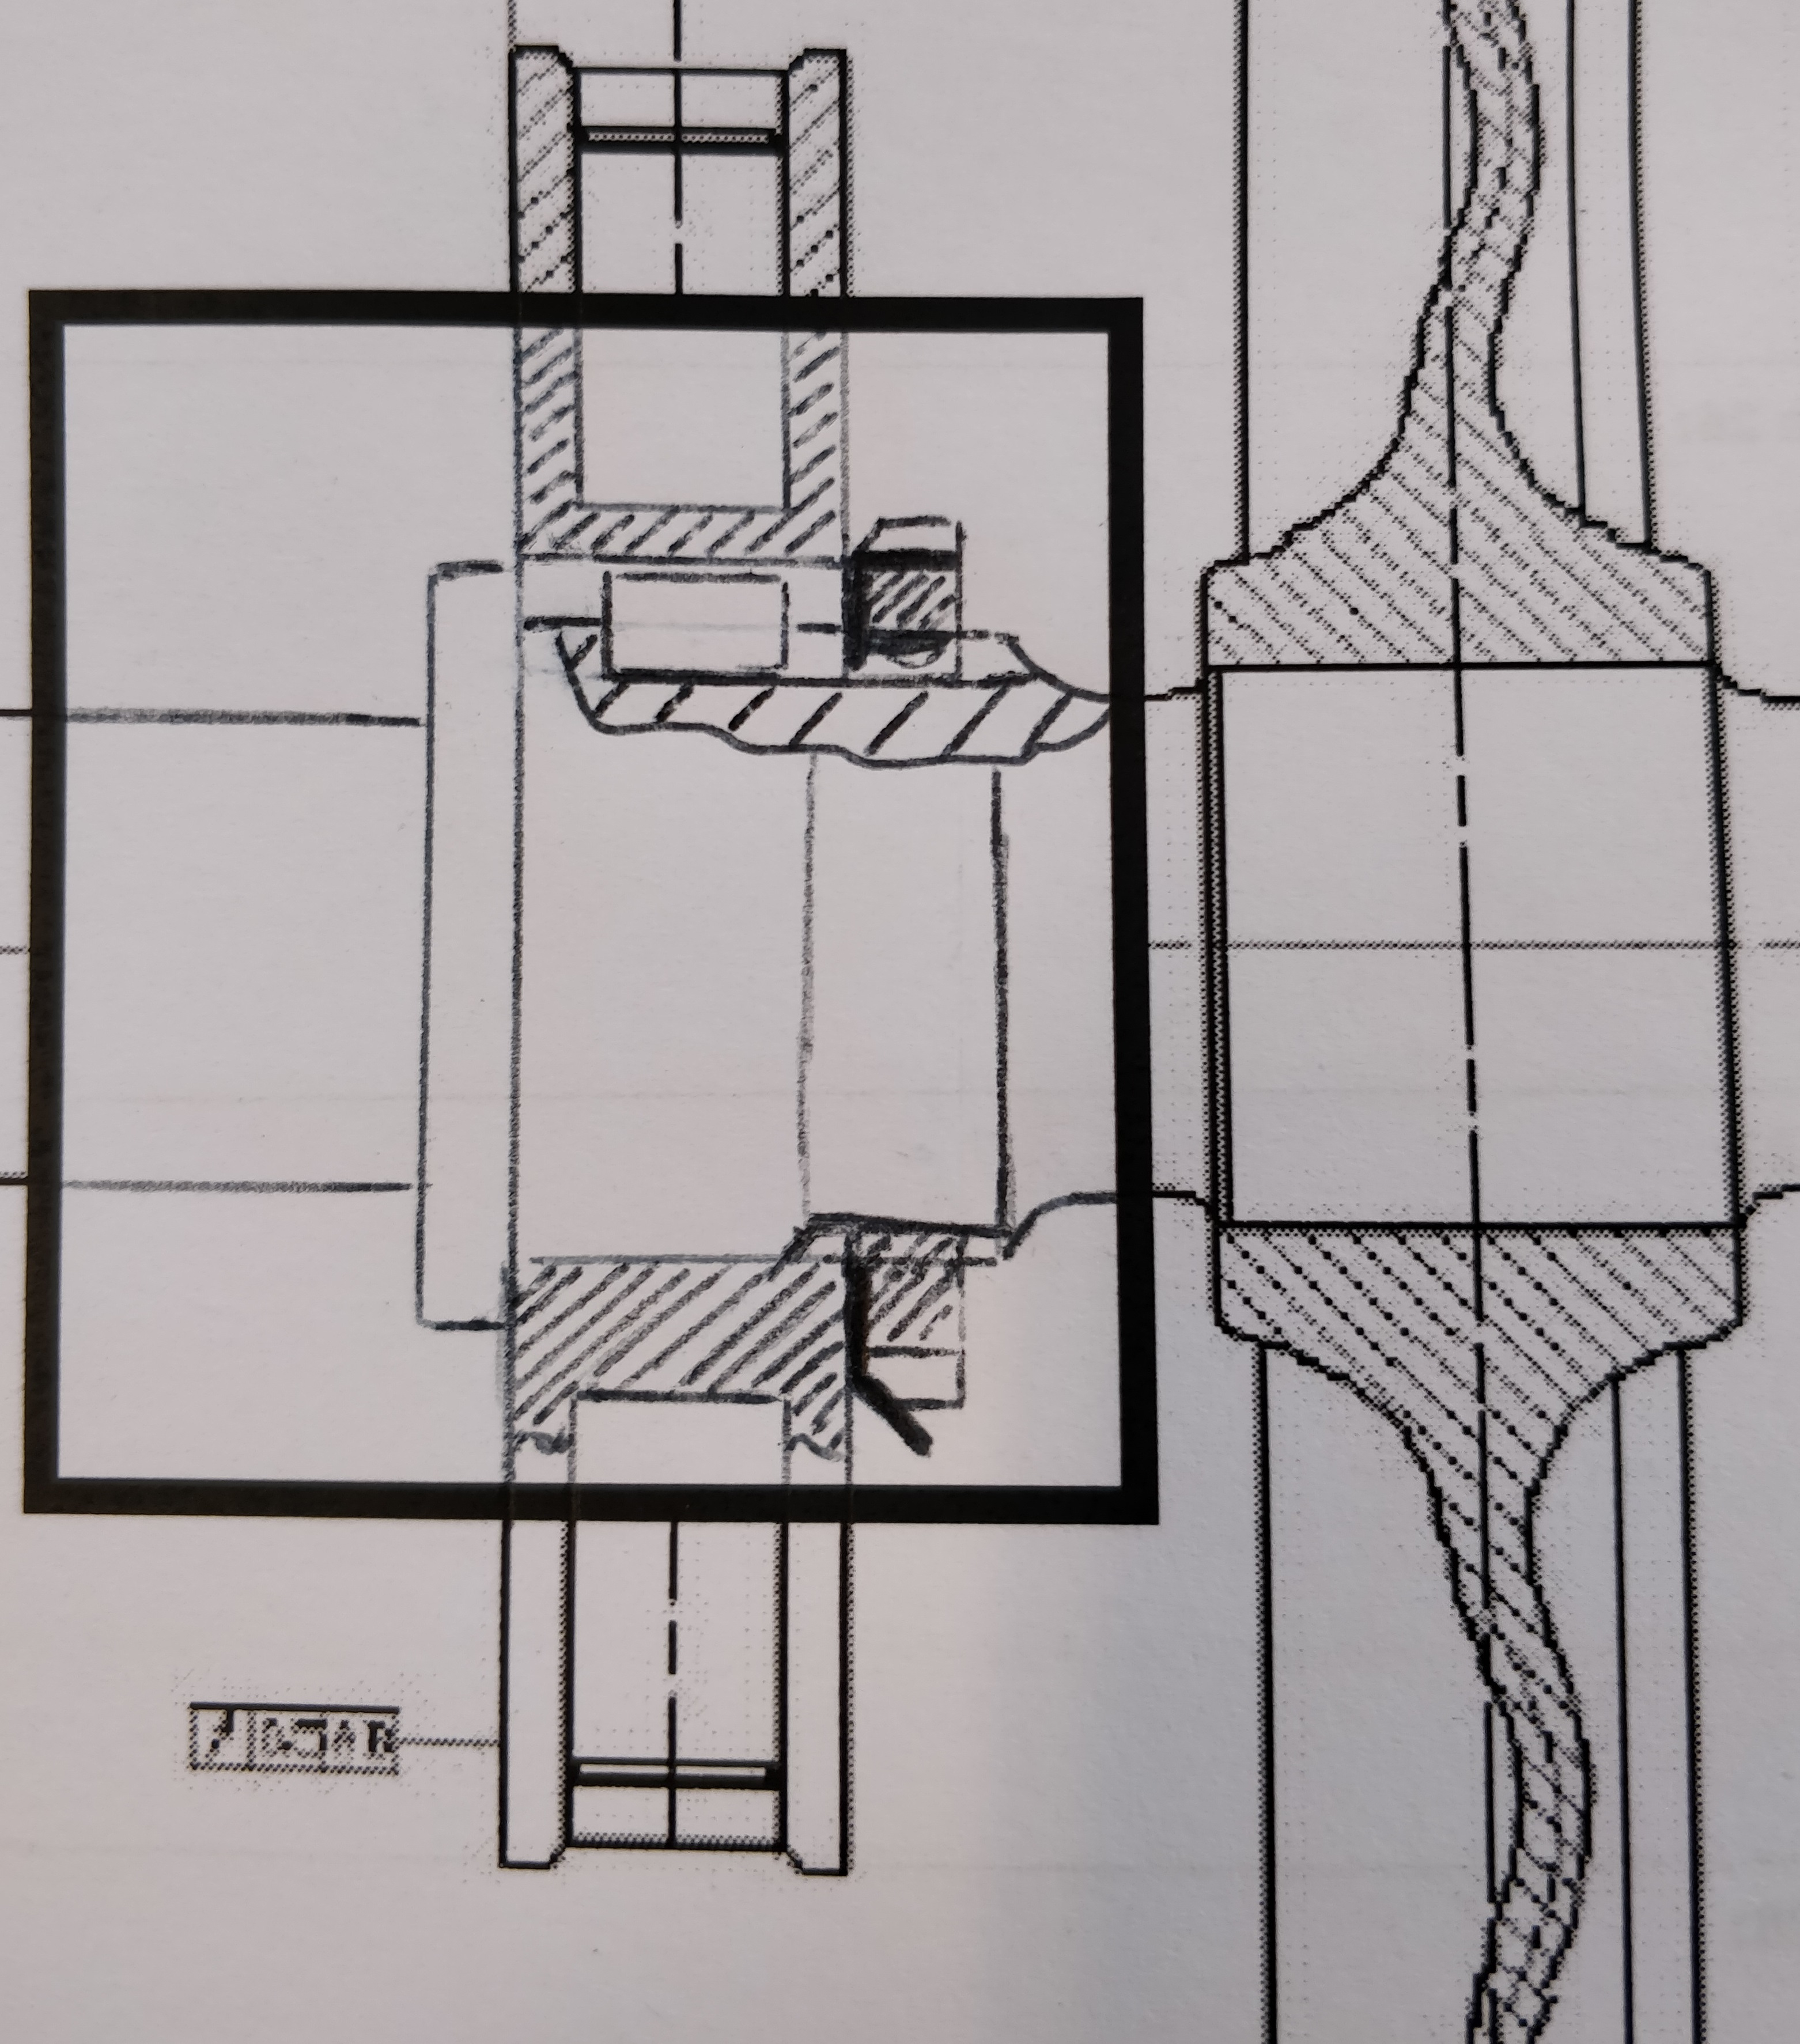
\includegraphics[width=0.5\linewidth]{img/dessin_cor}
\end{center}}


\end{document}

